
%\documentclass[final,twocolumn,number,sort&compress]{elsarticle}
%\documentclass[review]{elsarticle}
%\documentclass[preprint,12pt,authoryear]{elsarticle}
%\documentclass[review,number,sort&compress]{elsarticle}
\documentclass[final,times,3p,twocolumn]{elsarticle}


\usepackage{lineno,hyperref}
\usepackage{upgreek}
\usepackage{xcolor}
\usepackage{textcomp}

%\modulolinenumbers[5]

%\journal{Journal of \LaTeX\ Templates}

\linenumbers 
%\modulolinenumbers[5]

%\journal{Journal of \LaTeX\ Templates}

%%%%%%%%%%%%%%%%%%%%%%%
%% Elsevier bibliography styles
%%%%%%%%%%%%%%%%%%%%%%%
%% To change the style, put a % in front of the second line of the current style and
%% remove the % from the second line of the style you would like to use.
%%%%%%%%%%%%%%%%%%%%%%%

%% Numbered
%%\bibliographystyle{model1-num-names}

%% Numbered without titles
%\bibliographystyle{model1a-num-names}

%% Harvard
%\bibliographystyle{model2-names.bst}\biboptions{authoryear}

%% Vancouver numbered
%\usepackage{numcompress}\bibliographystyle{model3-num-names}

%% Vancouver name/year
%\usepackage{numcompress}\bibliographystyle{model4-names}\biboptions{authoryear}

%% APA style
%\bibliographystyle{model5-names}\biboptions{authoryear}

%% AMA style
%\usepackage{numcompress}\bibliographystyle{model6-num-names}

%% `Elsevier LaTeX' style
\bibliographystyle{elsarticle-num}
%%%%%%%%%%%%%%%%%%%%%%%
\journal{NIMA}

\begin{document}

\begin{frontmatter}
\title{The CLAS12 Micromegas Vertex Tracker}

\author{A. Acker} 
\author{D. Atti\'e}
\author{S. Aune}
\author{J. Ball}
\author{P. Baron}
\author{Q. Bertrand}
\author{D. Besin}
\author{T. Bey}
\author{F. Boss\`u}
\author{R. Boudouin}
\author{M. Boyer}
\author{G. Christiaens}
\author{P. Contrepois}
\author{M. Defurne}
\author{E. Delagnes}
\author{M. Gar\c con}
\author{F. Georges}
\author{J. Giraud}
\author{R. Granelli}
\author{N. Grouas}
\author{C. Lahonde}
\author{T. Lerch}
\author{I. Mandjavidze}
\author{O. Meunier}
\author{Y. Mouden}
\author{S. Procureur}
\author{M. Riallot}
\author{F. Sabati\'e}
\author{M. Vandenbroucke}
\author{E. Virique}

\address{IRFU, CEA, Universit\'{e} Paris-Saclay, 91191, Gif-sur-Yvette, France}

\begin{abstract}The High Threshold Cerenkov Counter (HTCC) is one of the detector systems of the CLAS12 spectrometer, and is used to generate fast trigger signal in electron experiments. The HTCC is installed in front of the R1 Drift Chambers and introduces a minimal amount of additional material within working acceptance. The HTCC is one unit whose core component is a multifocal mirror that consists of 60 lightweight composite ellipsoidal mirrors. It is important that the HTCC provides efficient coverage of the CLAS12 acceptance with no gaps or overlaps. In order to achieve this, each sector of the CLAS12 spectrometer is covered by 2 identical half-sector mirrors that focuses Cerenkov light on eight phototubes. The HTCC has a total of 48 channels with Electron Tubes 9823QKB PMTs that have a 5" quartz face plate to detect Cerenkov light. The system provides a high rejection of charged $\pi$-mesons and low background noise for reliable identification of scattered electrons. The details of the design, construction, calibration, and performance results of the HTCC are presented in the following paper. 

\end{abstract}

\end{frontmatter}

\section{Introduction}
\label{introduction}

The physics program for CLAS12 in Jefferson Lab's Hall B requires the use of electron beams of various energies and currents that impinge
upon on targets ranging from liquid hydrogen to lead. A significant part of the physics program includes running with polarized targets that 
require a rastered beam on the target. In order to extract experimental observables, accurate measurements of the beam charge and 
polarization are required. Also, for safe and efficient operation of a large, open acceptance spectrometer, proper shielding and a stable beam 
with a small lateral size and minimal beam halo are needed. 

The Hall-B beamline is designed to satisfy experimental requirements and provide necessary controls and monitoring 
of the electron beam properties for safe and efficient operation of CLAS12. The key set of parameters required by experiments with CLAS12 
is listed in Table \ref{tab:beam_par}. The main challenges for the beamline setup are the open acceptance of CLAS12 and the close proximity 
of various sensitive detectors to the target and beam. Such challenges were successfully overcome in Hall B in the past for CLAS \cite{CLAS} 
experiments and the Heavy Photon Search (HPS) experiment \cite{HPS}.

 \begin{table}[htb]
 \centering
 \begin{tabular}{|c|c|c|}
\hline
Parameter & Requirement &Unit \\ \hline 
$E$ &  $\le 11$& GeV \\ \hline
$\delta p/p$ & $< 10^{-4}$ & \\ \hline 
Current & $<~500$ & nA \\ \hline
Current instability & $\sim 10$ &\% \\ \hline 
$\sigma_x $, $\sigma_y$&$< 300$& $\mu$m \\ \hline 
Position stability &$< 200$ &$\mu$m \\ \hline
Divergence& $< 100$& $\mu$rad \\ \hline 
Beam halo ($> 5\sigma$) &$< 10^{-4}$& \\ \hline
Beam polarization &$> 0.85$& \\ \hline
\end{tabular}
\caption{Nominal required Hall B beam parameters.} 
\label{tab:beam_par}
\end{table}

A few key modifications to the beamline \cite{HPSBeamline} used during the lower-energy run of the HPS experiment have been introduced 
in order to establish high-quality physics beams in Hall B and run CLAS12 at the design luminosity of $10^{35}$ cm$^{-2}$s$^{-1}$.  
Additions to the beamline for high-energy running of CLAS12 include a new intermediate beam dump upstream of the hall, a cryogenic 
target system, shielding downstream of the target to protect CLAS12 detectors from electromagnetic backgrounds, and the M{\o}ller 
polarimeter for beam polarization measurements.   

%\begin{figure*}[t]
%\begin{center}
%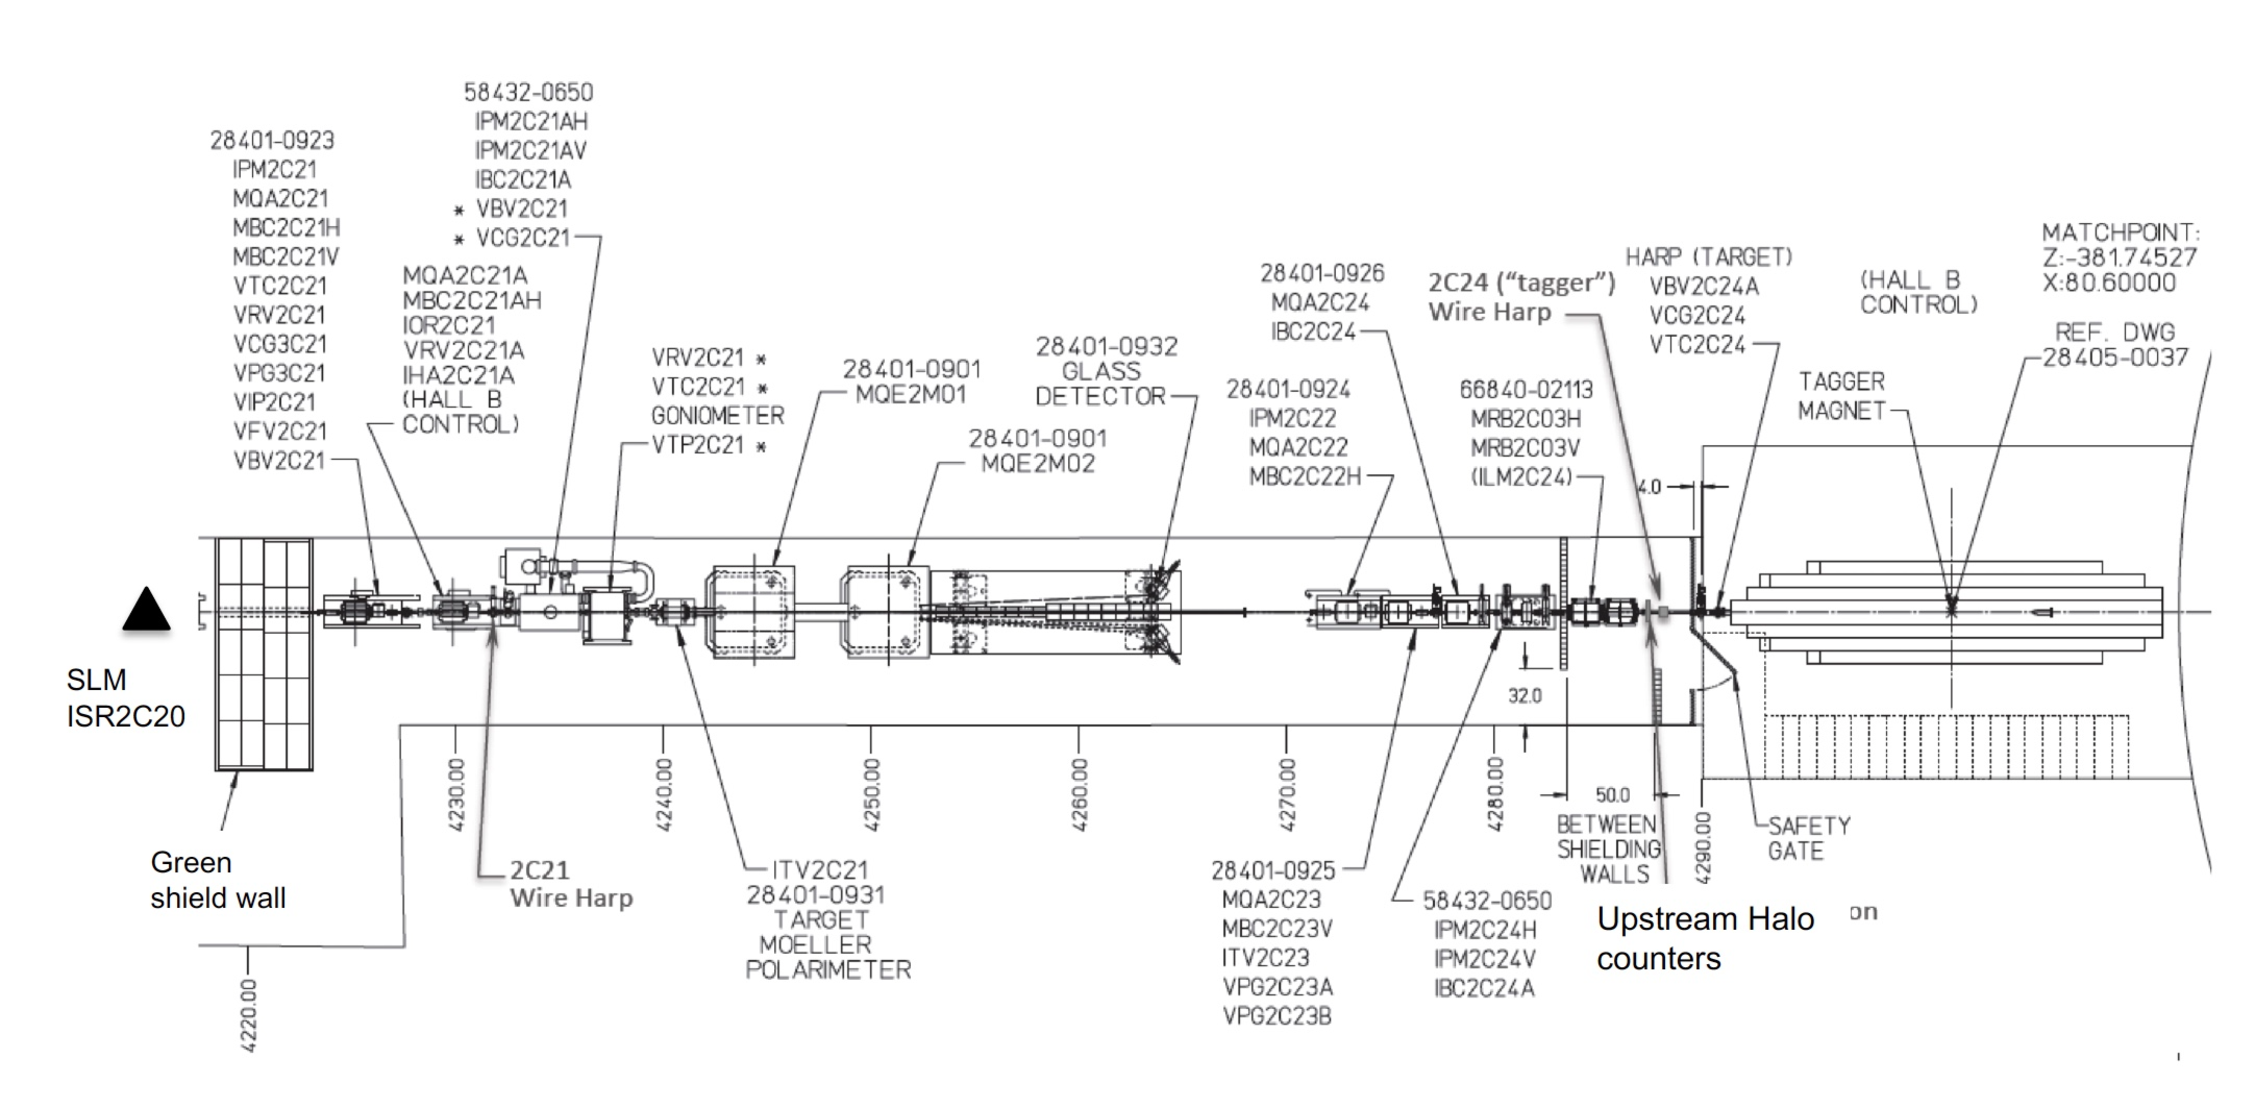
\includegraphics[width=1.\textwidth]{upstream_tunnel.pdf}
%\caption{Overhead view of the 2C beamline in the tunnel upstream of Hall B. {\color{red} Not the final figure.}}
%\label{fig:upstream}
%\end{center}
%\end{figure*}

 
This paper will discuss the design of the Hall-B beamline for CLAS12, and its performance during the 2018 experimental run. It will review the 
beamline instrumentation used to measure and monitor beam parameters and to protect CLAS12 detectors against errant beam motion. As will 
be demonstrated, excellent quality and stability of the CEBAF beams, coupled with the Hall-B beamline protection systems, allowed running the 
CLAS12 detector at the design luminosity.



\section{Detector Layout}

\subsection{The Calorimeter (FT-Cal)}

The FT-Cal has to fulfill demanding requirements in terms of: radiation hardness, light yield, shower containment
(small radiation length and Moliere radius), fast recovery time, and good energy and time resolution.

The electron energy resolution is a crucial factor to determine precisely the photon energy and to ensure the
exclusivity of the measured reaction via the missing mass technique. However, since we are interested in low-energy
electrons and high-energy photons, the energy resolution on the latter is significantly better than the resolution on
the electron\footnote {For example, an electron energy resolution of 2\% (at 1~GeV) would result in an energy
  resolution of $\sim$0.2\% for the corresponding 10~GeV photon, allowing the use of the missing mass technique
  for most of the reactions of interest.}. The FT-Cal should have a fast recovery time ($\tau\sim$ 10~ns) to sustain
high rates with small pile-up effects and to provide the scattered electron interaction time with good accuracy
($<$1~ns) in order to reject background and to identify the relevant signals via coincidence with CLAS12. Due to the
expected high rate from electromagnetic background, the calorimeter should be highly segmented in the transverse
direction. The size of each detection element should be comparable with the characteristic transverse size of the
electromagnetic shower (Moliere radius) to contain the shower produced by incident electrons to a few readout cells,
thus minimizing rates and pile-up. Finally, the photodetectors for the light read out should work  in a sizable magnetic
field and fit within the available space. Thus, standard photomultipliers (PMTs) cannot be used while photodetectors
based on semiconductors, e.g. avalanche photodiodes (APDs), have been shown to meet the required criteria. 

To match the necessary requirements, lead tungstate (PbWO$_4$) was chosen as the scintillating material and
Large-Area APDs (LAAPDs) as the readout sensors. A similar  combination was used in the CMS-ECal~\cite{CMS-ECal},
CLAS-IC~\cite{CLAS-IC}, and PANDA-EMC~\cite{PANDA-ECal} calorimeters. Lead tungstate has a fast scintillation
decay time (6.5~ns), a small radiation length (0.9~cm), and small Moliere radius (2.1~cm). The drawback of limited
light emission (about 0.3\% of NaI(Tl)) has been mitigated by using cooled PbWO$_4$ Type-II crystals (as for the
PANDA-EMC), matched to large-area photosensors to obtain a factor of four more light per MeV of deposited energy
than the original CMS-ECal crystals.

With this design an energy resolution of the order of ($2\% /\sqrt{E\textrm{(GeV)}} \oplus 1\%$) is expected.
Other crystals, such as LSO/LYSO or the very recent LaBr, share almost all of the good specifications of
PbWO$_4$ with a light yield more than 100 times larger. However, the lack of extensive studies on radiation
hardness and the limited experience in the manufacturing procedures excluded them from consideration as an
alternative.

\begin{figure}[th!]
\centering 

\includegraphics[width=0.85\columnwidth]{fig/dummy.png} 
\caption{FT-Cal} 
\label{fig:ft-cal-geometry} 
\end{figure}

\subsubsection{Geometry and Coverage}

The FT-Cal is made from 332 $15\times 15\times 200$~cm$^3$ parallelepiped PbWO$_4$ Type-II crystals
arranged around the beamline with full azimuthal angular coverage ($0^\circ < \phi < 360^\circ$)  and small
forward angles acceptance ($2^\circ < \theta < 5^\circ$). The crystals are placed with their long side parallel to
the beamline to form a ring. Figure~\ref{fig:ft-cal-geometry} shows the crystal assembly. 

\subsubsection{PbWO$_4$ Crystals}

The FT-Cal PbWO$_4$ Type-II crystals were produced by the Shanghai Institute of Ceramics, Chinese Academy
(SICCAS). Since the light yield ($LY$) increases when lowering the temperature $T$ according to 
$dLY/dT \sim 3\%/^\circ$C, the calorimeter is stabilized in temperature and operated at
$T \sim 0^\circ$C. Lower temperatures were not considered due to significant complications in the
mechanical/thermal design, the reduced resistance to radiation,  and the decay time degradation of the cooled
PbWO$_4$. The length of the crystals (20~cm - corresponding to $\sim$22 radiation lengths) was chosen to
minimize the longitudinal loss and to match the available clearance.

The size of the crystal front face of 15~mm $\times$ 15~mm provides a pixelization in the transverse plane of
the PbWO$_4$ crystals consistent with the Moliere radius. All crystals were characterized using the ACCOS
(Automatic Crystal quality Control System) facility at CERN~\cite{accos}. The geometrical dimensions, as well as the
optical properties such as the longitudinal and transverse transmission and the relative light yield, were determined
for each of the crystals. Samples that were outside of the required specifications were rejected and replaced by the
manufacturer. 

The absolute $LY$ (number of detected photoelectrons per MeV deposited) was found to be $N_{pe}=220\pm 20$
at $T=0^\circ\textrm{C}\pm 0.5^\circ\textrm{C}$. For this measurement the crystal was wrapped on 5 of its faces
with 3M Vikuiti reflective film and read out by a Hamamatsu S8664-1010 LAAPD operated at a gain $G$=150
connected with optical grease on the exposed face. 

The scintillation decay time is also sensitive to the temperature. The time constant was measured using the
{\it Start-Stop} or {\it Delayed-Coincidence} method at different temperatures. As expected, an increase in the
decay constant was observed by decreasing the temperature. At $T=0^\circ\textrm{C}\pm 0.5^\circ\textrm{C}$, we
found $\tau=13.5\pm 0.6$~ns ($\tau_1=11.6\pm 0.5$~ns and $\tau_1=13.0\pm 0.2$~ns) when a single (double)
exponential form was used to fit the data.

\begin{figure}[th!]
\centering 
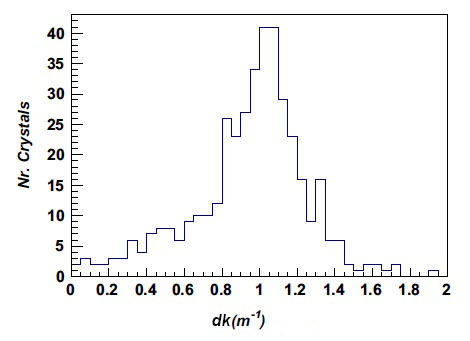
\includegraphics[width=0.85\columnwidth]{./fig/dk.jpeg} 
\caption{Histogram of the radiation-induced absorption coefficient, $dk$, for all SICCAS FT-Cal PbWO$_4$ crystals.}
\label{fig:dk} 
\end{figure}

The radiation hardness of the crystals was measured by irradiating them with a dose of 30~Gy of low-energy photons
using a $^{60}$Co source at the Strahlenzentrum of Giessen University~\cite{radhard}. The longitudinal transmission
was measured before and after the irradiation, calculating the variation as a function of the wavelength. The radiation
hardness of the crystals was quantified by the radiation-induced absorption coefficient defined as:

\begin{equation}
dk = \frac{1}{L}\frac{T_{bef}}{T_{irr},}
\end{equation}

\noindent
where $T_{bef}$ is the light transmission at 420~nm, the peak of the PbWO$_4$ emission spectrum, measured before
irradiation, and $T_{irr}$ is the light transmission at the same wavelength after irradiation for crystals of a given
length $L$. Crystals exhibiting greater levels of radiation damage to light transmission have higher values of $dk$.
All 332 crystals assembled in the FT-Cal were individually characterized: on average we found 
$T_{bef}$(420~nm) = $61.5 \pm 0.2$ ($\sigma=3.2$) and $T_{irr}$(420~nm) = $50.8 \pm 0.5$ ($\sigma=4.9$). 
The resulting $dk$ distribution is shown in Fig.~\ref{fig:dk}. These measurements were used to optimize the position
of each crystal in the calorimeter, placing the crystals with the highest radiation resistance, and therefore lowest
$dk$, in the areas where the highest radiation dose is expected.

\begin{figure}[th!]
\centering 
\includegraphics[width=1.0\columnwidth]{./fig/apd5.eps} 
\caption{Intrinsic gain of one APD as a function of the bias voltage and of the temperature.}
\label{fig:G-V-T} 
\end{figure}

\subsubsection{Light Readout and Electronics}
\label{sec:ftcalread}

The FT-Cal uses $10 \times 10$~mm$^2$ (model Hamamatsu S8664-1010) LAAPDs to read out the PbWO$_4$
scintillation light. APDs are very compact devices (only a few mm thick), have a large quantum efficiency at the
PbWO$_4$ light peak emission (420~nm), and  are insensitive to magnetic fields. The main disadvantage is that,
due to their low intrinsic gain ($\sim$50-200), the output signal is too small to be directly acquired, and needs to
be amplified by a suitable circuit. APDs also need to be operated at a controlled temperature to avoid variations in
gain and noise, but this does not represent a major complication since the crystals also are required to be stabilized
in temperature. Each sensor used in the FT-Cal has been characterized by measuring its gain as a function of the
applied bias voltage at a given temperature using an automated  custom facility (see Ref.~\cite{celeAPD} for more
details). The typical gain behavior $G(V_{Bias},T)$ is shown in Fig.~\ref{fig:G-V-T}. The working point (bias voltage)
was chosen in order to have the chosen gain ($G=150$) in a reasonably stable region for small variation of the biasing.
Silicon photomultiplier (SiPM) readout was not considered due to their limited dynamic range, which is not suitable for
spectroscopic applications, and the limited experience (in term of reliability, radiation hardness, stability in time, etc.)
in their use in large experiments at this time.

The APD current signal is converted to a voltage pulse that is transmitted to the subsequent electronics chain via a
trans-impedance amplifier (i.e. an amplifier that converts an input current pulse into an output voltage pulse, without
performing any time integration). This amplifier has been developed in collaboration with the Service Electronique
pour la Physique (SEP) of the Institut de Physique Nucl{\'e}aire (IPN) in Orsay. The amplifier ENC \footnote{The ENC,
  equivalent noise charge, is defined as the charge transported by an input signal giving, at the output of the amplifier,
  a signal whose amplitude is equal to the RMS of the output noise.} was measured at the operating temperature of
T=0$^\circ$C,  with ENC=8200$\pm$100 $e^-$ (RMS) for the nominal gain of $G=1800$ {\color{red} (CORRECT
  TO ACCOUNT THE FINAL GAIN WAS SET TO 600)}. The amplified signal is read out using the custom JLab flash
ADC VME board (a 16-channel, 12-bit, 250~MHz digitizer; referred to as the FADC250). The measurement
of the full waveform allows for the derivation of both the charge and time of the hit with the required  accuracy.

\subsubsection{Light Monitoring System}

Lead tungstate scintillating crystals are known as an appropriate material for use in total absorption shower
detectors. Unfortunately, although relatively radiation tolerant, their light output is reduced when exposed to 
radiation and recovers when the radiation source is removed. Further complications arise because at the same
irradiation intensity, changes in light output may vary from one crystal to another. In order to maintain the intrinsic
energy resolution, the crystals have to be continuously monitored and, if necessary, re-calibrated by changing the
supply voltage. The monitoring system should be able to test the response over time of the whole chain: crystal,
APD, read-out electronics. Among the different possible options (radioactive source, laser, and LED) we used an
LED-based Light Monitoring System (LMS). In spite of the need for thermal control, LEDs offer considerable
advantages: matching with crystals is simpler than for lasers, since each crystal can have a LED in front of it and
the arrangement of power lines and electrical connections is less critical than for optical fibers. The main
disadvantage is related to the complexity of the electronic circuitry: to cover a large light intensity range while
maintaining a good timing, each LED needs a separate driver, which leads for a calorimeter of significant size, to
a large number of electronic circuits.

With LEDs it is possible to obtain a shape and a duration of the monitoring-light flash that is similar to the features
of the crystal scintillation light. In fact, the emission spectrum of the monitoring light can be chosen to be similar to
the radio-luminescence spectrum of PbWO$_4$, the effective optical path length for monitoring light in the crystal
can be matched to the average path length of the scintillation light produced by an electromagnetic shower, and the
pulse length can be tuned to reproduce the PbWO$_4$ scintillation decay time. We chose a blue light LED with
wavelength close to the 430~nm emission peak of the PbWO$_4$ crystal, where radiation damage may have the
maximum effect. Each crystal is equipped with a separate LED, located on its upstream face, at the
opposite end with respect to the light sensors and electronics. The intensity can be varied in the range from 500 to
100,000 photons, pulsed at a variable rate from 62~Hz to 8~kHz, with a pulse rise time of $\sim$1~ns and a time
jitter of less than 200~ps. The system has been designed to work in the temperature range from -25$^\circ$C
to +30 $^\circ$C. The LEDs placed in the closed environment of the crystal are kept at constant temperature with an
accuracy of $\Delta T$ = 0.1$^\circ$C. The LED monitoring system is split in two boards: one containing the control
logic and the LED driver circuits, and the other, mounted in front of the FT-Cal crystals, hosting the LEDs. The two
boards are connected via a board-to-board connector that allows the required flexibility to match the FT-Cal
geometry and positioning. The LED drivers are controlled by an on-board PIC32 micro-controller accessible remotely
via Ethernet. Each LED is individually set by a programmable length and intensity pulse. The system is triggered by
an internal clock or by an external signal. In both cases the trigger signal is available for a precise time reference. 

\begin{figure}[th!]
\centering 
\includegraphics[width=1.0\columnwidth]{./fig/dynamics.eps}
\caption{Number of photoelectrons as a function of the LED driver current. The corresponding energy per crystal
  ranges from 10~MeV to 10~GeV.}
\label{fig:LEDperf1} 
\end{figure}

\begin{figure}[th!]
\centering 
\includegraphics[width=1.0\columnwidth]{./fig/timing.eps}
\caption{Time resolution (measured as the time difference of the trigger signal and the PMT pulse) as a function of
  the LED light intensity.}
\label{fig:LEDperf2} 
\end{figure}

The performance of the LED driver has been measured by coupling a single monitoring channel to a PMT. The
performance of the system is reported in Figs.~\ref{fig:LEDperf1} and \ref{fig:LEDperf2}, where the measured
number of photoelectrons as a function of the LED current and the measured time resolution as a function of the
number of photoelectrons are shown\footnote{The time resolution is defined as the width ($\sigma$) of the time
  difference distribution between the trigger signal and the PMT output.}. Rescaling the results to take into account
the APD readout and the crystal $LY$/MeV, the equivalent energy ranges from 10~MeV (500~phe) to 10~GeV
(500k~phe) perfectly matched to the expected energy collected by each crystal. A time resolution of 100~ps is
reached at high light intensity. The long term stability of the system has been measured over a 100-hr run at
$T=+18^\circ$C. The stability of each individual channel was found to be in the range of 2\%; when the ratio of
the two channels is considered, the stability is at a level of a few parts per thousand.

\subsubsection{Slow Controls and Interlocks}

The FT-Cal slow controls are part of the CLAS12 EPICS system~\cite{daq}. The APDs need to be reverse-biased
with a positive high-voltage power source. The APD intrinsic gain depends on the bias voltage with
$\frac{1}{G}\frac{\Delta G}{\Delta V} \sim4 \%$ and, therefore, the power supply needs to be stable in time, with
low output noise. We chose the CAEN A1520P board designed for the CMS electromagnetic calorimeter. The power
supply fulfills  all our requirements in terms of dynamic range, linearity, and noise. Each board is equipped with 12
independent channels that each control a group of ten APDs with relative gain variations not greater than 3\%.

The amplifiers used in the FT-Cal need to be operated with +5~V and -5~V. The power consumption from each of the
two voltage sources is approximately 70~mW, almost independent of the event rate, giving a power consumption of
$\sim$140~mW per board, for a total of 56~W for a 400-channel calorimeter. The full FT-Cal is powered by a
Wiener MPOD MPV8008L power supply. Sensing feedback is implemented to compensate the voltage drop across the
connecting cables.

Temperature regulation is provided by a Lauda XT150 chiller unit. This is a self-regulating unit and does not require
external feedback, however, the settings and monitored parameters are sent to EPICS for recording via a
{\it streamDevice} module. The FT-Cal temperature is monitored by a set of PT100 thermoresistors located at
different positions within the crystal assembly and read by a {\it cRio} module, which is part of the interlock system.
The flow of nitrogen gas, which is purged in the preamplifier area to prevent moisture build-up at low temperature,
is measured with a flowmeter and monitored by the same {\it cRio} system. The latter is also used to read the output
of two humidity sensors located in the preamplifier area. 

The {\it cRio} system is the main component of the interlock system that was designed to provide a fast shutdown
mechanism for all critical components in case abnormal conditions are detected. The parameters that are monitored
are the FT-Cal temperatures, the nitrogen flow, and the humidity. If any of the measured values is found to be
outside user-defined ranges, the system disables the FT-Cal high voltage (HV) and low voltage (LV) crates and stops
the chiller to prevent any damage to the detector or surrounding elements.

\subsubsection{Mechanical Design}

The mechanical design of the calorimeter is driven by three considerations: minimization of the empty spaces between
crystals, cooling to $0^\circ$C, and optimal coverage of the required acceptance without interference with the rest
of CLAS12.

\begin{figure}[th!]
\centering 

\includegraphics[width=1.0\columnwidth]{./fig/sc-assembly.eps}
\caption{Single crystal assembly: from the left (front) to the right (back), the PEEK support that holds the nose with
  the LED housing, the crystal wrapped in 3M Vikuiti reflective film, the LAAPD in the PEEK housing, and the
  preamplifier.}
\label{fig:crystalassembly} 
\end{figure}

The building blocks of the calorimeter are the individual lead-tungstate crystals. Each crystal is
$15\times 15\times200$~mm$^3$, for a weight of 370~g. Each crystal is optically coupled to a LAAPD on its
back face and to an LMS LED on its front face for calibration. To achieve the maximum light collection efficiency,
the APD covers almost the entire area of the downstream end of the crystal, so the LED for monitoring has to be
mounted on the upstream end. This reflects onto the mechanical design of the single crystal assembly as a monolithic
self-supporting element made of the crystal itself, the APD, the reflective wrapping, and the crystal support
structure. To avoid dead volume in the detector, the mechanical support for each crystal is provided only by the
wrapping. We chose 3M Vikuiti reflective film. This material is non-conductive, has a reflectivity higher than
aluminized Mylar and, if properly heat-formed, can hold the weight of a crystal. The reflective film is glued on the
sides of a pair of front/back PEEK custom-machined blocks that hold the LAAPD and the LED, respectively.
Figure~\ref{fig:crystalassembly} shows a CAD rendering of the single crystal assembly from the front PEEK
support to the preamplifier.

\begin{figure}[th!]
\centering 
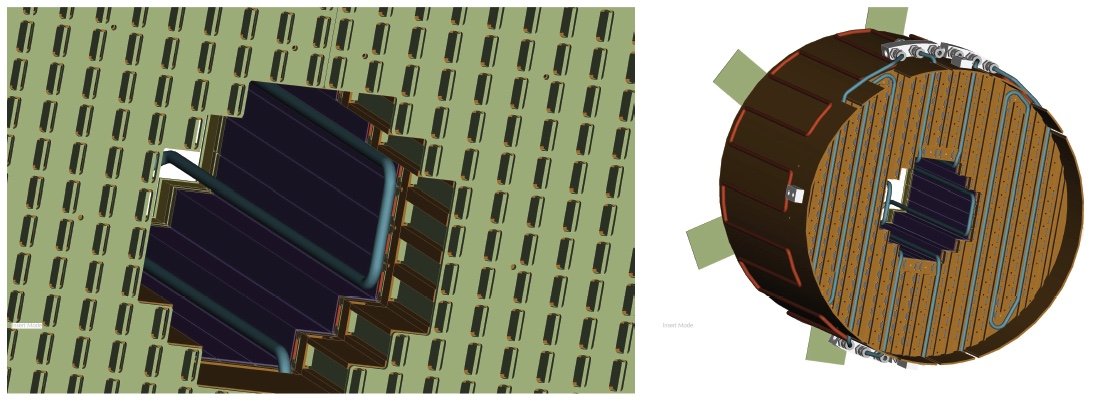
\includegraphics[width=1.0\columnwidth]{./fig/raff.jpeg}
\caption{The copper thermal/grounding shield for the FT-Cal with the cooling pipes shown.}
\label{fig:piping} 
\end{figure}

The crystal assemblies are installed in a matrix to provide complete shower containment for electrons in the FT-Cal
angular acceptance. Two copper plates, placed in front of and on the back of the crystals, define the positioning for
the crystal assemblies. On the APD side, the preamplifiers, one for each crystal, are connected to the readout
motherboard, which is designed to provide power distribution and signal collection for each channel. The mechanical
structure allows for the replacement of individual preamplifiers if needed. The front and back copper plates are
connected by a copper cylinder on the outside and by an inner copper shield to form a closed vessel that surrounds
the crystal matrix to provide proper grounding and the required thermal stability and uniformity. Cooling is provided
by 5-mm diameter copper pipes installed on the outside of the vessel as shown in Fig.~\ref{fig:piping}. A CAD section
view of the complete calorimeter is shown in Fig.~\ref{fig:calsec}.

\begin{figure}[th!]
\centering 
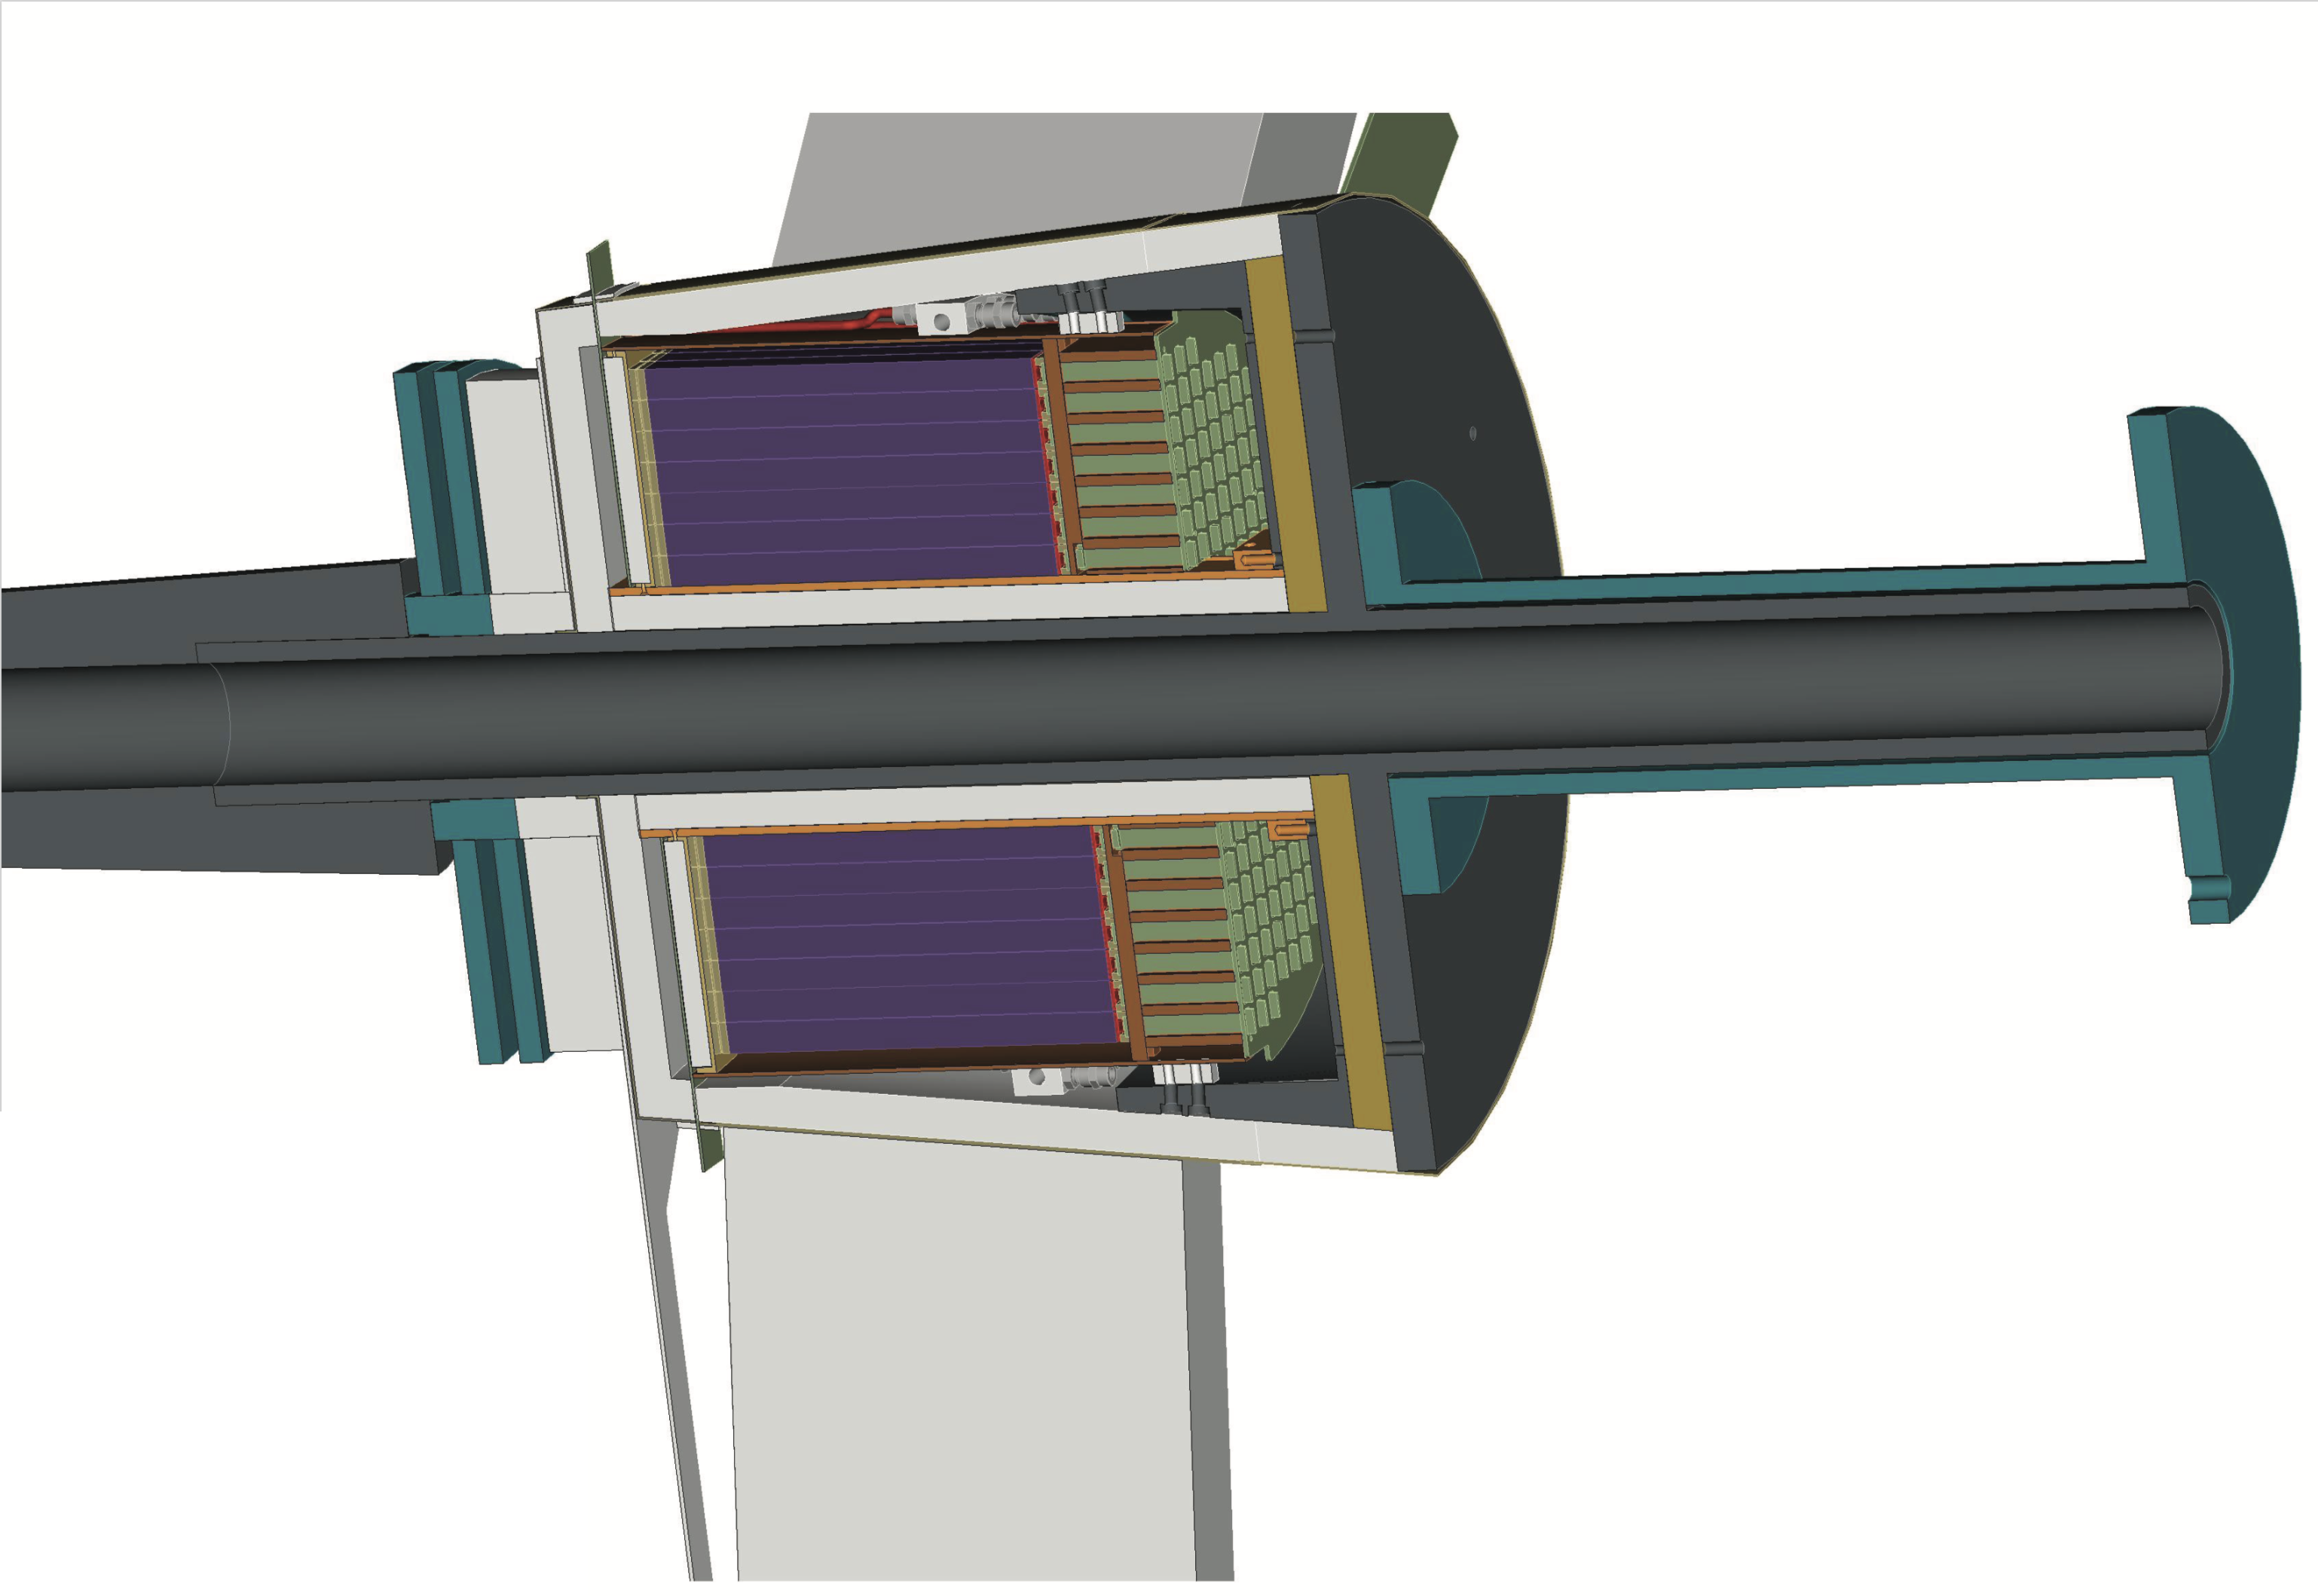
\includegraphics[width=1.0\columnwidth]{./fig/section.png}
\caption{Cross section of the FT calorimeter: in purple, the crystals, upstream the PEEK forward blocks and the
  forward copper plate, downstream the rear copper plate, the preamplifiers (in green), and the readout
  motherboard (in white), {\color{red} in light gray and yellow, part of the insulation.}}
\label{fig:calsec} 
\end{figure}

The FT calorimeter has been designed to operate between 0$^\circ$C and room temperature. The FT-Cal cooling is
achieved via circulation of coolant in the circuit attached to the rear copper plate and on the inner and outer copper
vessels. The cooling system was designed to compensate the heat load in the region surrounding the FT, taking into
account 20~mm of insulating foam (polyisocianurate thermal conductivity 0.024~W/mK) and from the amplifiers, which
dissipate $\sim$50~W. The insulation is less effective between the calorimeter and the inner tungsten pipe that
holds the entire FT (see Section~\ref{sec:integration}) because of the limited space for the insulation and the
presence of the support structures that bring the overall thermal conductance in that region to 0.056~W/mK.

During the design phase, Finite Element Analysis calculations were performed to optimize the cooling circuit and the
insulation parameters in order to reach the design temperature and uniformity. These studies indicated that the
coldest part of the external calorimeter enclosure is the tungsten cone that is expected to stabilize at a temperature
just above the dew point. Measurements performed after the calorimeter assembly confirmed these results.

\subsection{The Hodoscope (FT-Hodo)}

The primary aim of the FT-Hodo is to discriminate between photons and electrons that produce the electromagnetic
shower in the calorimeter. Specifically, electrons are identified by hits in the hodoscope array that are correlated
in both position and time with a cluster observed in the calorimeter. The FT-Hodo is comprised by an array of 232 plastic
scintillator (Eljen-204) tiles segmented in two layers to suppress contributions from the splash-back of the
electromagnetic shower created by events depositing energy in the FT-Cal. The scintillators provide fast timing and
sufficient resistance to radiation damage for use in the high-rate and high-dose environment of the FT. The geometry
and readout of the hodoscope are constrained by the surrounding apparatus. Specifically, the device is positioned
upstream of the FT-Cal, fitting into a circular disk of diameter 330~mm and 42~mm depth. The readout is achieved
using $3 \times 3$~mm$^2$ Hamamatsu S13360-3075PE SiPMs (50\% photon detection efficiency for 450~nm
photons) coupled to 5-m-long clear optical fibers (Kuraray clear-PSM with attenuation length $>10$~m), which are
fusion spliced to $\sim$30~cm long wavelength shifting (WLS) Kuraray Y11 fibers (attenuation length of $> 3.5$~m),
embedded in the scintillator tiles. The splicing induces a photon loss of less than 2\%, where the use of optical fibers
allows the captured light to be transported with a light loss of less than $\sim$40\% over the 5~m path to the SiPM.
This readout design of the FT-Hodo addresses the need to minimize material in the detector acceptance, to operate
in regions of high magnetic fields produced by the CLAS12 solenoid and torus magnets, and to tolerate the high
background radiation environment. 

Each layer of the FT-Hodo is comprised of 44 15~mm$\times$15~mm (P15) and 72 30~mm$\times$30~mm (P30)
scintillators arranged as shown in Fig.~\ref{Fig:FTHodoLayout}. The upstream and downstream layers utilize 7-mm
and 15-mm thick scintillator tiles, respectively. The upstream (thin) layer is employed to reduce photon conversion in
the FT-Hodo, while the thicker layer provides the signal with the most accurate timing information for the event. To
increase the number of scintillation photons collected from each tile, four WLS fibers were embedded in the P30
tiles and 2 in the P15 tiles. In addition, the WLS fibers were glued with Bicron BC-600 glue (CHECK Epotek 301-2)
inside diagonal holes to maximize the path length in the scintillator and to allow for the tiles to be arranged without
any dead space between the elements. Each tile was polished and painted with two layers of Bicron BC-620 reflective
paint for the sides and 3 layers for the scintillator faces and secured in position on the surface of a 2-mm-thick
plastic support board. There is a 9~mm clearance for each layer for routing the optical fibers to the readout
electronics through a $\Delta$-shaped sheathing on the bottom end of the FT-Hodo. The front and back faces are
covered by light-proof carbon fiber material that is screwed onto supporting structures made out of hexagonal
plastic spacers (15-mm wide and 22- or 15-mm tall depending on the layer). This results in a total detector thickness
of 44~mm. A 1-mm thick plastic strip traces the outer contour of the FT-Hodo and is glued on the spacer supports.
Figure~\ref{Fig:CADFT-Hodo} shows a CAD drawing of the FT-Hodo showing half of one layer of tiles, the location
of the plastic supports for the light-proofing structure, and the plastic strip.  

\begin{figure}[th!]
\centering 
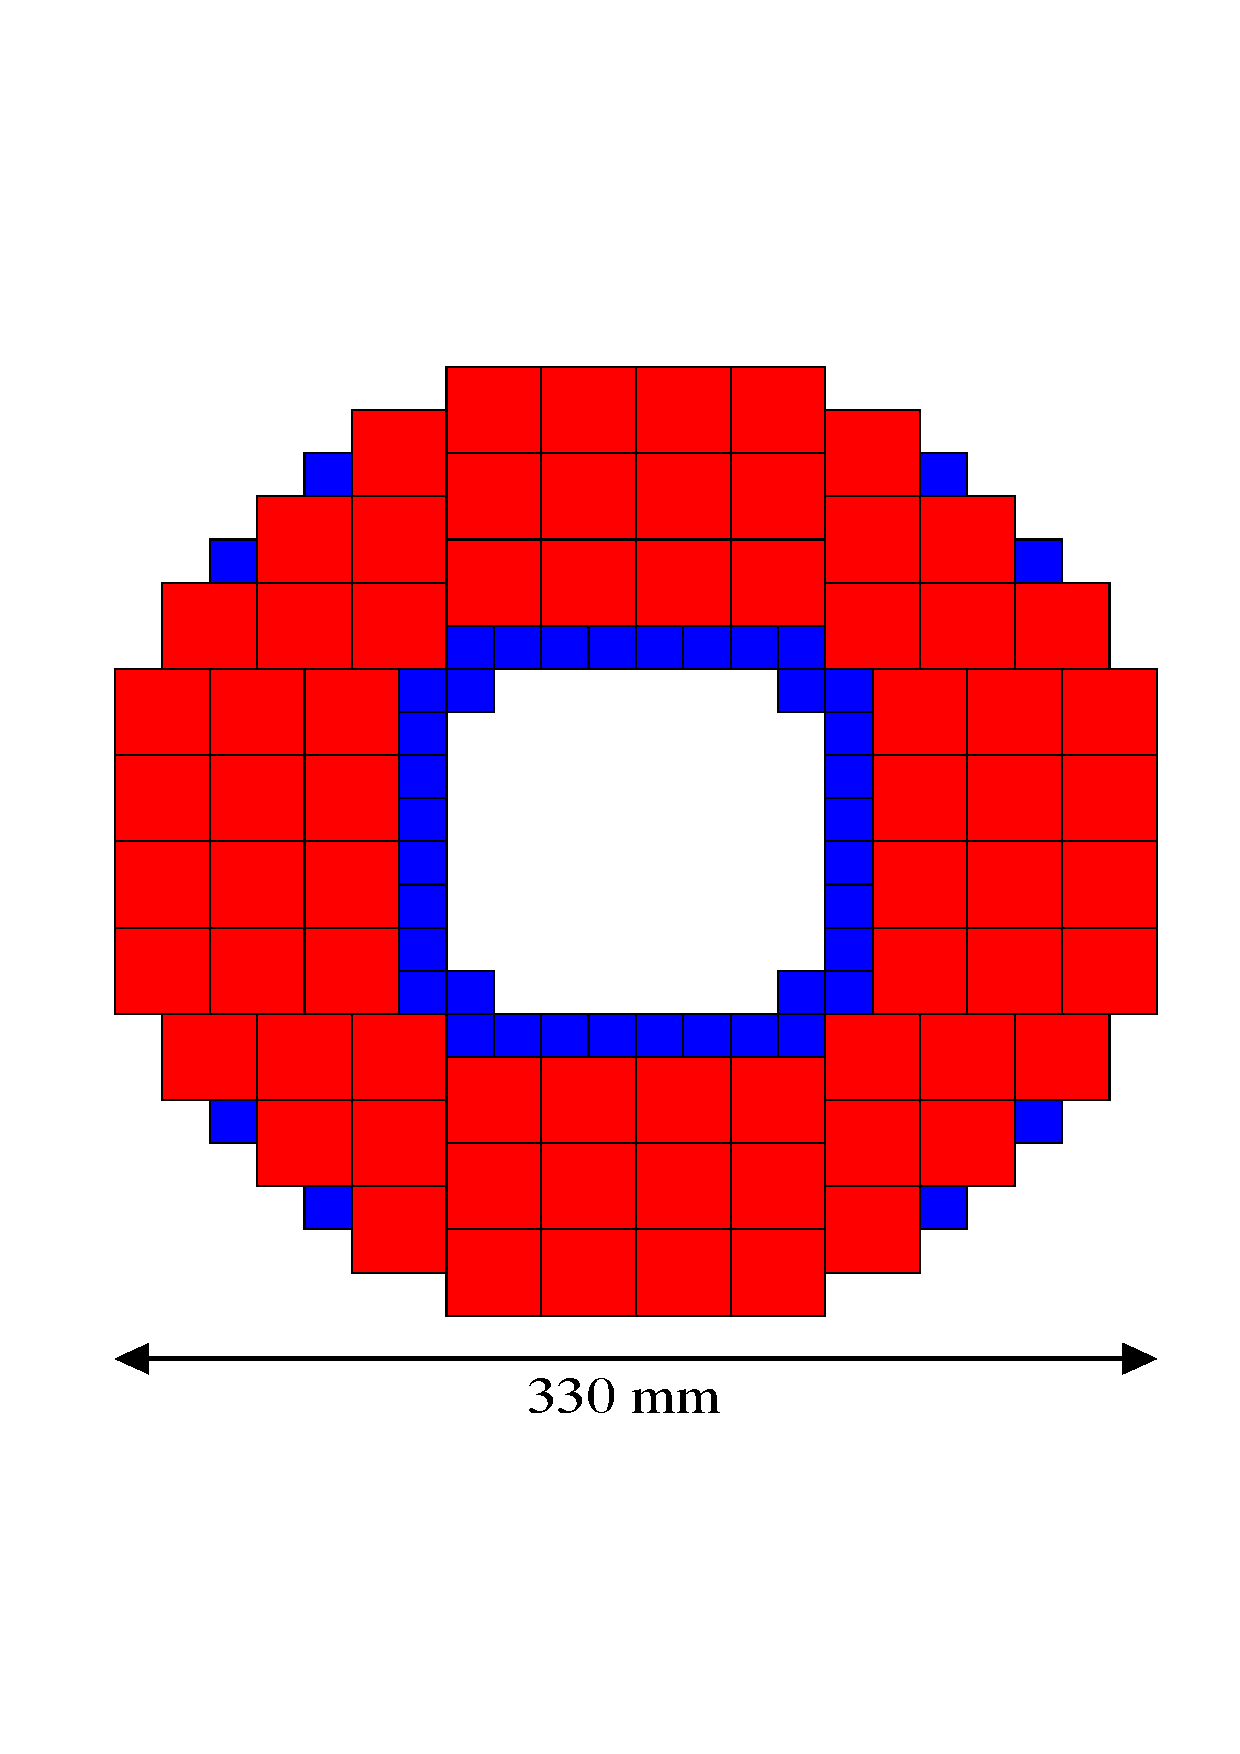
\includegraphics[width=0.85\columnwidth]{./fig/FTHodoLayout.pdf} 
\caption{The arrangement of plastic scintillator tiles in the FT-Hodo. The blue (red) squares represent the
  15~mm$\times$15~mm (30~mm$\times$30~mm) tiles for each layer.} 
\label{Fig:FTHodoLayout} 
\end{figure}

\begin{figure}[th!]
\centering 
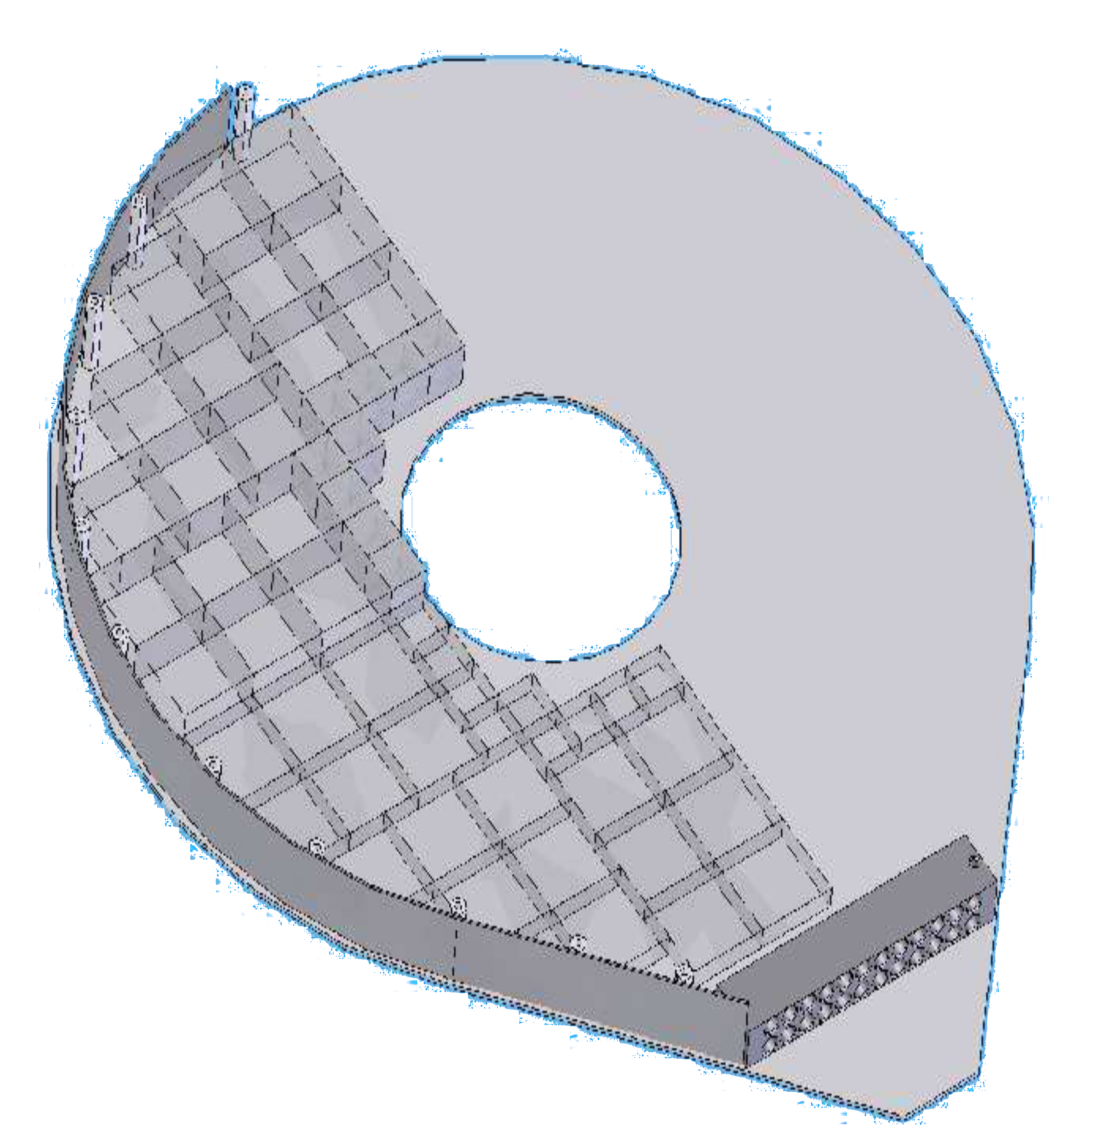
\includegraphics[width=0.85\columnwidth]{./fig/CADFT-Hodo.pdf} 
\caption{CAD drawing of the FT-Hodo showing half of layer 1, the location of the plastic spacers, and the plastic
  strip that traces the outer contour. WILL BE REPLACED WITH BETTER RESOLUTION FIGURE} 
\label{Fig:CADFT-Hodo} 
\end{figure}

With the typical maximum radiation doses determined through Geant4 simulations with realistic beam and target
parameters, and without the shielding effects of the M{\o}ller cone (see Section~\ref{sec:integration}), the
FT-Hodo will experience a light loss of 20\% in the WLS fibers after 3.5 years, whereas the plastic scintillators will
experience a light loss of 20\% after 300~years~\cite{ft-tdr}. Both scintillators and fibers also show natural
annealing processes, which can effectively compensate for the radiation damage~\cite{ft-tdr}.  

The analog signal from the SiPM is fed directly to a custom-designed preamplifier board designed by the
INFN-Genova Electronics Group. The boards host 8 independent channels each coupled to a SiPM and are mounted
in pairs in the slots of a custom crate, mechanically compatible with the VME standard. The 16 SiPMs connected to
each pair of boards are mounted on a mezzanine printed circuit board, which distributes the bias HV to each SiPM
and collects their signals for the amplifier inputs. The schematic of one channel of the SiPM amplifier board,
excluding the HV bias network is shown in Fig.~\ref{Fig:FTHODOAmpBoard}. The first stage is based on a bipolar
junction NPN transistor in a common base configuration, while the second is composed by a OPA694 operational
amplifier in a non-inverting configuration. The two BRF92 transistors have been chosen since they are low-noise
transistors with a high cut-off frequency and good stability. The two stages are coupled together with a 100~nF
capacitor to remove the DC component of the signal from the second transistor. The amplifier is coupled to the
output connector through a 100~nF capacitor and a 50~$\Omega$ resistor to remove any DC component from the
last stage and to match the impedance of the output cable. 

\begin{figure}[th!]
\centering 
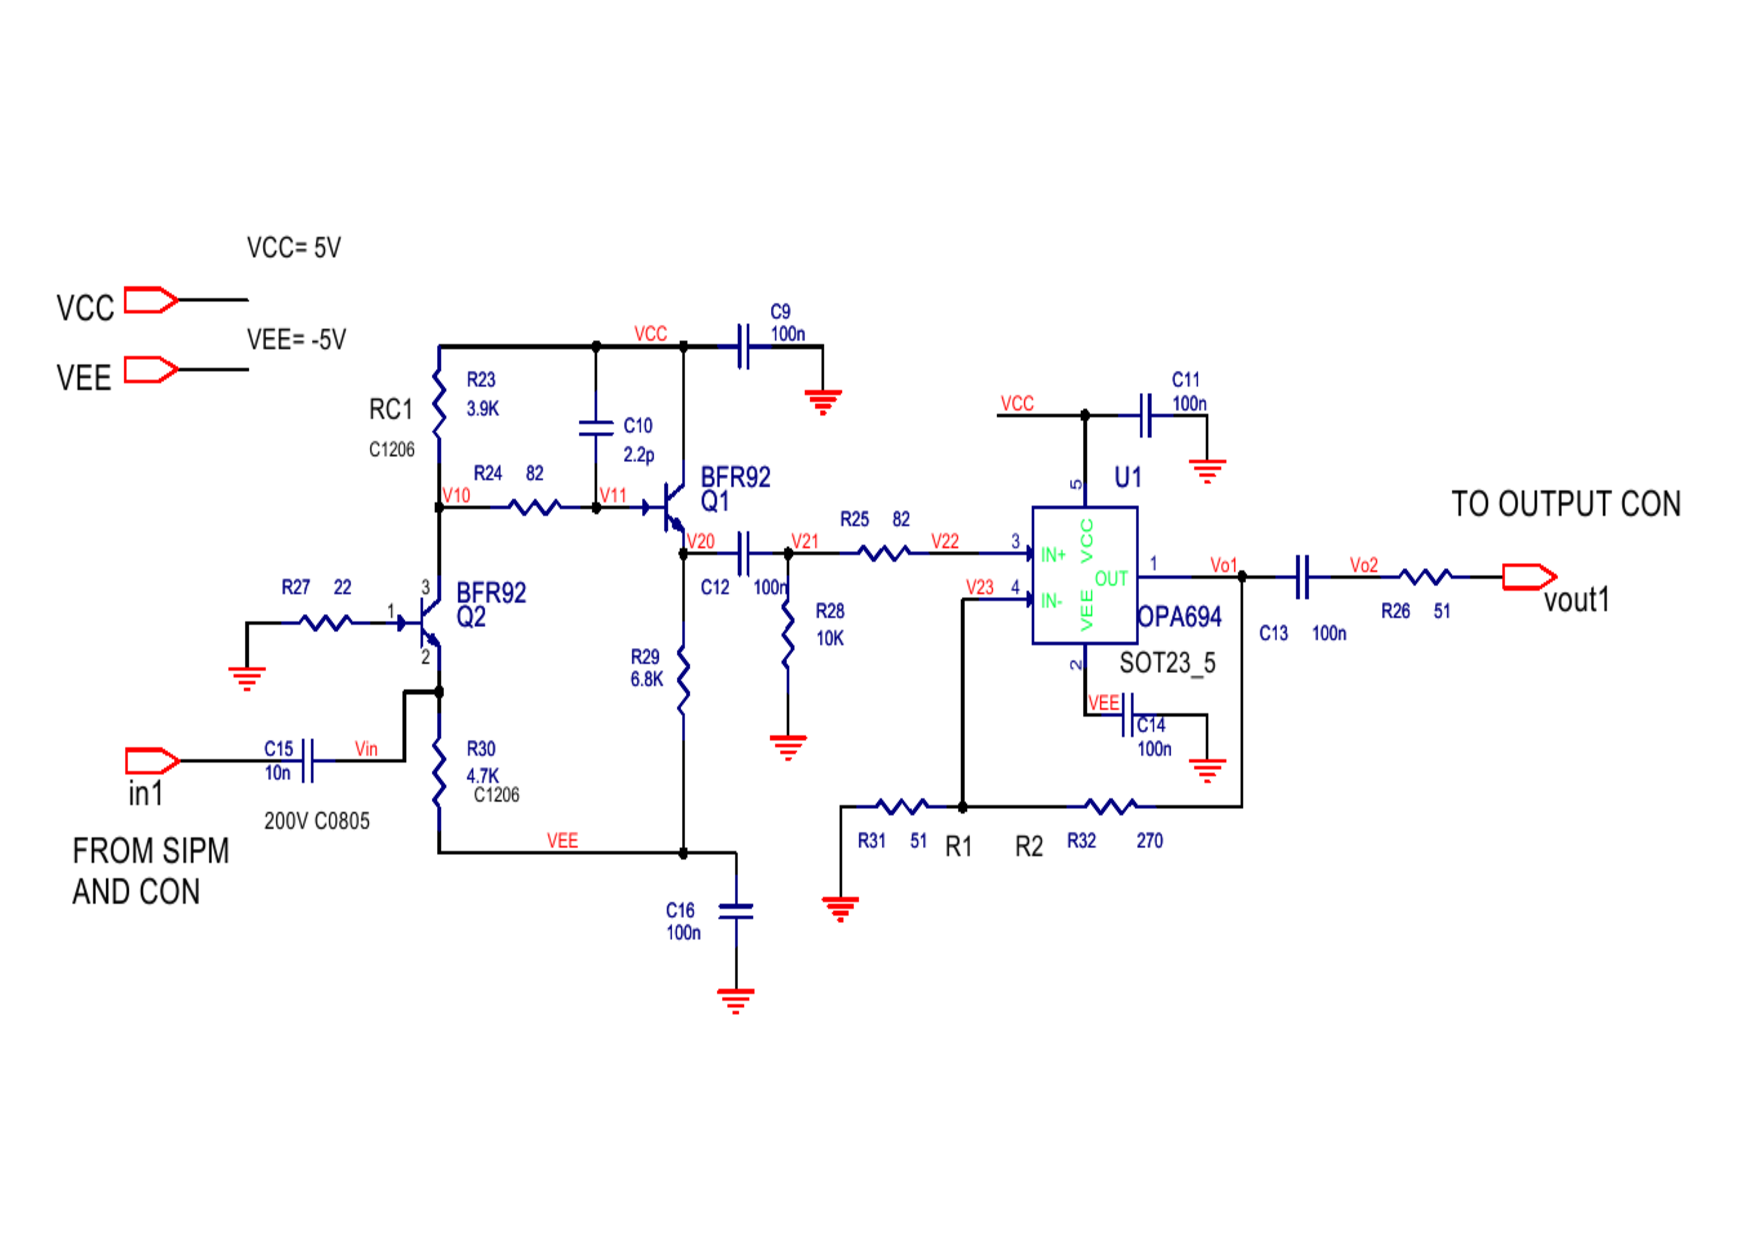
\includegraphics[width=1.0\columnwidth]{./fig/FTHODOAmpBoard.pdf} 
\caption{Schematic of a single channel of the amplifier board for the SiPM.} 
\label{Fig:FTHODOAmpBoard} 
\end{figure}

The signal from each SiPM after amplification is continuously digitized by the JLab FADC250 boards and, if the
trigger condition is satisfied, samples are stored for further analysis. The data acquisition and slow controls system
for the FT-Hodo are similar to the FT-Cal (see Section~\ref{sec:ftcalread} for more details). The SiPMs operate
with a bias voltage of 50-55.5~V, which is provided by three CAEN A1737P HV boards. 30 independent HV channels
are used to operate each SiPM board that hosts 8 sensors. These groups of 8 SiPMs were selected according to their
gain. The HV distribution to the groups of 8 SiPMs is implemented on the mezzanine boards that also hosts a
compensation circuit to allow for the independent regulation of each SiPM bias voltage up to a maximum of 0.4~V. The
low voltage system used for the FT-Hodo is the same as the one used for FT-Cal. Controls of both the HV
and LV for the detector are provided by the CLAS12 EPICS slow controls system~\cite{daq}. Similarly to the FT-Cal,
the status of the critical components, in this case the temperature of the preamplifier crate, is incorporated into
the interlock system that is programmed to disable the HV and LV crates if abnormal conditions are detected.

\subsection{The Micromegas Tracker (FT-Trk)}

For a precise determination of the scattered electron angle, a tracker complements the FT-Cal and FT-Hodo
detectors. The FT-Trk uses the same technology adopted by the CLAS12 central and forward Micromegas detectors.
We refer to Ref.~\cite{mm} for a detailed description of  these devices. In this section we describe the specific
design of the FT-Trk.

\begin{figure}[th!]
\centering 
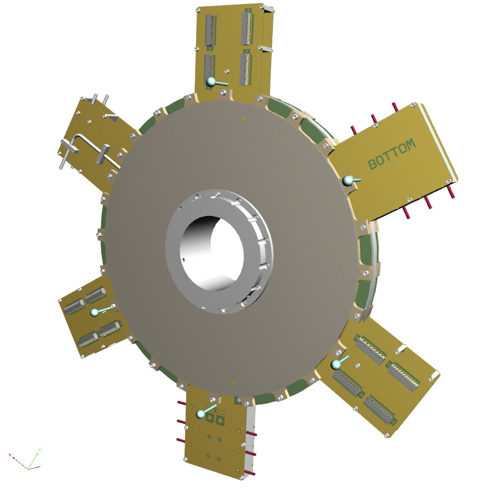
\includegraphics[width=1.0\columnwidth]{./fig/fttrk_layout.png}
\caption{3D view of the upstream face of the FT-Trk Micromegas tracker equipped with front-end electronics.}
\label{fig:ft-trck} 
\end{figure}

Two double-layers of Micromegas detectors are located in front of the hodoscope, in the space between the FT
and the High Threshold Cherenkov Counter (HTCC)~\cite{htcc}. The two detectors are indeed a good compromise
to achieve an efficient background rejection and track reconstruction with a low material budget. Each layer is
composed of a double-faced Micromegas disk built on a common printed circuit board (PCB). Each side of the PCB
displays strips, the downstream strips being perpendicularly oriented to the upstream strips. This particular geometry
enables the determination of the $(x,y)$ coordinates (perpendicular to the beam $z$-axis) of a track. To limit the
number of electronics channels, the pitch chosen was 500~$\mu$m, which leads to a resolution better than
$500/\sqrt{12} \sim 150$~$\mu$m. A drift space of 5~mm, together with an amplification gap of 128~$\mu$m,
provides good efficiency. The two double-layers, centered on the beam axis, cover polar angles from 2.5$^\circ$ to
4.5$^\circ$ with an active area defined between a 70~mm inner radius and a 143~mm outer radius. The total number of
channels is 3072. Figure~\ref{fig:ft-trck} shows the CAD implementation of the detector. The FT-Trk readout uses
the same data acquisition scheme adopted for the CLAS12 Barrel Micromegas Tracker (BMT)~\cite{mm}, which consists of
a Front-End Unit (FEU) and a Back-End Unit (BEU). 

The front-end electronics are responsible for signal preamplification, shaping, buffering during the trigger generation
process, data digitization, and compression. Due to the limited space available, the front-end electronics are designed
to be placed off-detector. Micro-coaxial cable assemblies connect the detectors and the front-end boards. The
non-amplified analog signals transit via the cable assemblies from the chambers to the front-end electronics. The
512-channel FEUs are housed in 4U crates attached to the FT-Cal mechanical supports and  located in the shadow of
the CLAS12 torus coils. The back-end electronics are responsible for data concentration, providing the interface to
the CLAS12 event building system and are the same units used for the BMT~\cite{mm}.

Each Micromegas layer is powered with 450~V for the micro-mesh and 1000~V for the drift electrode. The FT-Trk
front-end power supply is located 12~m away from the crates. The 15~W power produced by each crate is dissipated by
compressed air. An interlock system between the cooling infrastructure and the low voltage power supply prevents
powering the front-end crates when cooling is off. 

The gas used is a mixture of argon, isobutane (up to 10\%), and CF$_4$ (up to 5\%). The use of CF$_4$ ensures 
good time resolution (around 10-15~ns). The gas distribution system is the same one used by the BMT.

\section{Integration in CLAS12}
\label{sec:integration}

The FT mechanical design was driven by the geometrical constraints imposed by the other CLAS12 sub-detectors,
geometrical acceptance optimization, and performance optimization, taking into account cooling, material budget, and
front-end electronics location. The FT detects electrons scattered between $2.5^\circ$ and $4.5^\circ$ with respect
to the beam axis. To provide this acceptance, the FT calorimeter must cover down to $2^\circ$ and up to $5^\circ$ with
lead tungstate crystals to have a good containment of electromagnetic showers at the edges of the polar angular range.
Since no massive materials are allowed at angles larger than $5.5^\circ$, the crystals, cooling system, mechanical
supports, and tungsten shielding have been optimized in a very compact design. Outside of $5.5^\circ$ the only
materials are very low-density (35~kg/m$^3$) insulation and routing for cabling and services in the blind area of the
CLAS12 detector where the torus magnet coils are located.

The FT is built from several components that can be grouped as follows:

\begin{itemize}
\item{the inner tungsten pipe,}
\item{the tungsten cone acting as a M{\o}ller electron shield,}
\item{the FT-Trk tracker,}
\item{the FT-Hodo hodoscope,}
\item{the FT-Cal calorimeter,}
\item{the front-end electronics,}
\item{cabling and services.}
\end{itemize}

From the mechanical point of view, the most challenging aspect is the integration of the calorimeter, due to the
weight and fragility of the crystals, and the relative positioning and alignment of the FT components.

\subsection{Constraints from Other Sub-detectors}

The FT must be centered on the beamline between the HTCC and the first set of the DCs~\cite{dc}. The HTCC
can be retracted in the upstream direction to give access to the FT. In its operating position, the HTCC extends to
1730~mm downstream with respect to the nominal target center. This forms a plane that defines the upstream edge
of the space allowed for the FT. The first set of DCs is installed in front of the coils of the torus magnet, with an
inclination of $65^\circ$ with respect to the beam axis. The front-end electronics boards of the DCs define the
downstream border of the space allowance for the FT. The minimum distance of the DC boards from the beam axis
is $\sim$140~mm at 2280~mm downstream with respect to the nominal center of the target. Taking into account the
outside radius of the FT, including its insulation and the inclination angle of the DCs, the downstream face of the FT
cannot exceed $\sim$2150~mm with respect to the nominal center of the target.

The FT needs cabling and service routing for the gas and cooling lines. These services must be connected to the
outside of CLAS12. All services are installed in the blind area of the torus magnet coils, i.e. in the six azimuthal
slots extending radially from the beamline to the periphery. Each coil is $\sim$100-mm thick, which allows space
to host some front-end electronics for the FT, which must be close to the detectors.

The whole FT is attached to the torus magnet cryostat by a support structure with flanges on both ends. This is
needed both for the mounting sequence constraints and to avoid massive supports in front of the DCs. The support
structure consists of two concentric stainless-steel pipes connected by adjustment screws to allow for precise
alignment and positioning of the detector with respect to the beamline and the target position. A third tungsten
cylinder of smaller diameter is located inside the steel pipes to provide shielding from beam background. 

The FT is attached to the support structure via an inner tungsten pipe that is part of the calorimeter assembly
and is located inside the central holes of the FT detectors. This pipe is designed to support the entire weight of the
FT detectors and the additional shielding that is mounted upstream of the FT. Tungsten was chosen as the material
because, even if less resilient, is more rigid than stainless steel, thus reducing the gravitational sagging, and has
higher density and atomic number, i.e. better shielding properties. The FT-Cal is kept in position with respect to the
inner tungsten pipe via four radial supports, made of PEEK. PEEK was chosen because of its low thermal conductivity
(0.25~W/mK) and its relatively high tensile strength ($\sim$100~MPa). In addition, it features high radiation
hardness and excellent stability over a broad range of temperatures. Mounting rings of PEEK and aluminum,
respectively, are used to support and align the FT-Hodo and FT-Trk on the inner tungsten pipe.

Upstream of the FT, a tungsten cone is attached to the inner tungsten pipe to provide shielding from M{\o}ller
electrons produced by the interaction of the beam in the target~\cite{beamline}. Figure~\ref{fig:ftinclas12} shows a
section of CLAS12 with the FT in its operating position.

\begin{figure}
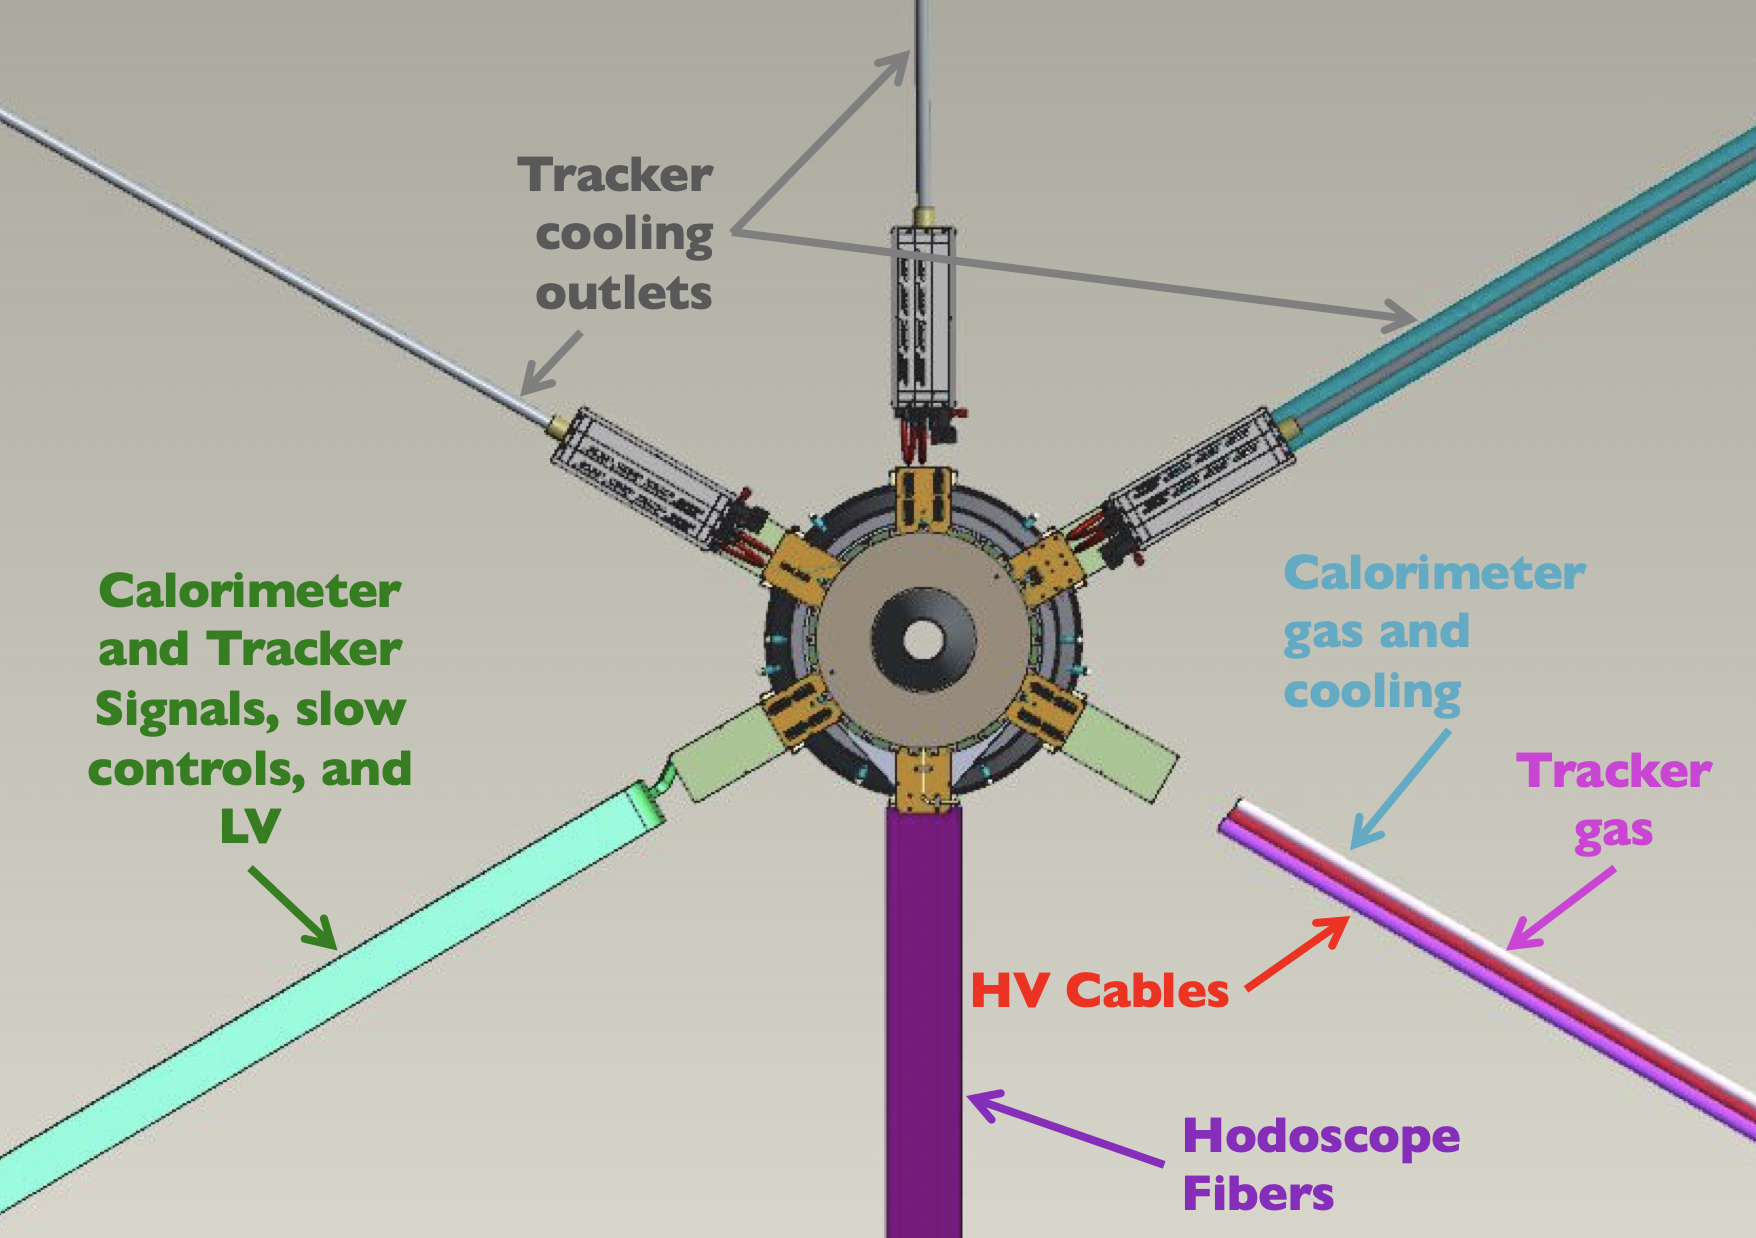
\includegraphics[width=1.0\columnwidth]{./fig/ft_cables.png}
\caption{Front view of the Forward Tagger with the routing of cables and services along the CLAS12 torus coils.}
\label{fig:integra}
\end{figure}

\subsection{Routing of Cabling and Services}

All services and cables necessary for the operation of the FT detectors are routed along the torus coils to minimize
the interference with the CLAS12 Forward Detector as shown in Fig.~\ref{fig:integra}. These include cables for signals
HV, LV, and slow controls, as well as piping for gas distribution and cooling of the three FT subsystems.

The cables and piping are routed along the direction of the magnet coils using appropriate rails. The
width and depth of the rails was chosen to be compatible with the space occupied by the DCs (both during
normal operation and maintenance) and the clearance between the HTCC and the CLAS12 Forward Detector.

\section{FT Prototypes}

Two prototypes of the FT-Cal, with 9 and 16 channels, respectively, were designed, assembled, and tested with
cosmic rays and electron beams to optimize and validate the detector design. Specifically, the prototypes were
used to check the single crystal mechanical assembly, the thermal performance, the front-end and read-out
electronics, and the electrical connections via a motherboard. The response to cosmic rays was studied for both
prototypes, while the response to electromagnetic showers was studied at Jefferson Lab (JLab) and the INFN
Laboratory Nazionali di Frascati (LNF) in Italy. The 9-channel prototype (Proto-9) was tested at JLab using 2-3~GeV
electrons deflected by the Hall~B tagger system~\cite{beamline},  while the 16-channel prototype (Proto-16) was
tested at the Beam Test Facility of LNF with a 0.5~GeV electron beam. Extensive simulations were performed
and compared to the results of the two sets of measurements. The main goals of the tests were:

\begin{itemize}
\item to measure the energy resolution as a function of the single-crystal threshold;
\item to measure the energy resolution as a function of $T$ (+18$^\circ$C, 0$^\circ$C, -10$^\circ$C, -25$^\circ$C);
\item to measure the time resolution;
\item to verify the system linearity;
\item to check rate performance;
\item to validate Monte Carlo (GEMC)~\cite{gemc} simulations;
\item to measure the electronic noise in realistic conditions;
\item to perform detailed studies of the electromagnetic shower signal: shower profile, APD signal shape, and test
  the filtering algorithm.
\end{itemize}

\subsubsection{The 16-Channel Prototype}
\label{par:proto-16}

The FT-Cal Proto-16 was built assembling 16 crystals in a $4\times4$ matrix (8 provided by the BTCP and 8 from
the RIINC company). Figure~\ref{fig:p16-whole} shows the Proto-16 components. Many mechanical and electrical
solutions tested on Proto-16 were then adopted in the final FT-Cal design. Due to the significant size of the crystal
matrix, the expected performance of Proto-16 in terms of energy resolution for showers generated at the center
of the 4$\times$4 matrix is similar to what was expected for the FT-Cal. Proto-16 was tested at the Beam
Test Facility (BTF)~\cite{btf} of LNF, using a 500~MeV electron beam. Data were taken in October 2012 to study
the prototype resolution as a function of the energy deposition and the calorimeter temperature. The BTF electron
beam is characterized by a repetition frequency of 50~Hz and a pulse duration of 10~ns. The beam intensity can be
varied by operating different sets of slits, selecting the number of electrons per bunch at the level of a single
particle. The prototype performance could therefore be studied as a function of the number of electrons 
simultaneously hitting the crystal matrix, i.e. of the detected energy.

\begin{figure}
\includegraphics[width=1.0\columnwidth]{./fig/p16-whole.eps}
\caption{Exploded view of the Proto-16 assembly. From left to right, the CAD drawing shows the motherboard, the
  system of copper rails holding the preamplifiers, the copper shield back plate, the crystal assembly, the copper
  shield front plate, and the LED board.}
\label{fig:p16-whole}
\end{figure}

Figure~\ref{fig:btf} shows the BTF experimental hall after the installation of Proto-16 and the associated equipment.
The detector was placed on a movable table that could be displaced in the $x$ and $y$ direction (transverse
plane) with a 0.1-mm accuracy. This feature was exploited to center the calorimeter with respect to the beam. A
plastic scintillator bar, read out by two PMTs, was placed in front of the beam pipe exit window and was used to
determine the arrival time of the electron within the 10-ns bunch duration. The data acquisition system, based on the
JLab CODA standard~\cite{daq}, was triggered by the radio-frequency (RF) signal of the Frascati accelerator. For
each trigger all of the signals of the Proto-16 crystal matrix and of the scintillator-bar PMTs were recorded by
CAEN VME boards. Both the Proto-16 and scintillator signals were sent to a passive splitter whose two outputs were
connected the 250~MHz FADCs and to leading-edge discriminators. The discriminator output was sent to pipeline
TDCs. The samples recorded by the FADCs in an 800~ns window were recorded for each trigger and analyzed offline
to evaluate the charge and time.

\begin{figure}
\includegraphics[width=1.0\columnwidth]{./fig/btf_oct12.eps}
\caption{Experimental setup of the Proto-16 test at the LNF Beam Test Facility (BTF). Beam comes from the right.
  On the left, the detector inside its case (black) is placed on a movable table to allow for centering of the calorimeter
  with respect to the beam. In front of the calorimeter, a plastic scintillator bar wrapped in black Tedlar is used to
  determine the arrival time of the beam electrons.}
\label{fig:btf}
\end{figure}

The conversion between charge and energy was first determined using cosmic ray measurements and then optimized
by studying the response of each crystal to 500~MeV electrons at the LNF-BTF. It is worth noting that the new
calibration constants were found to be within 5-10\% of the initial values determined during cosmic-ray data
taking. The total reconstructed energy  after the full calibration is shown in Fig.~\ref{fig:btf_etot} for an electron
multiplicity of the order of 1-2. The peaks corresponding to different bunch populations are clearly visible and well
separated. 

\begin{figure}
\includegraphics[width=1.0\columnwidth]{./fig/btf_etot_1876_2_6.eps}
\caption{The total energy measured by Proto-16 after calibration. The peaks correspond to different bunch
  populations and are clearly visible and well separated.}
\label{fig:btf_etot}
\end{figure}

\paragraph{Energy Resolution}

The mean values and widths ($\sigma$) of the peaks in the total reconstructed energy spectrum were analyzed to
check the system linearity and to determine the resolution. The measurements were performed by centering the
beam on the calorimeter to have the maximum containment of the electromagnetic shower.
Figure~\ref{fig:btf_linearity} shows the fitted peak position as a function of total energy in the beam bunch for an
APD gain of 150 and a PbWO$_4$ temperature of $18^{\circ}$C. The linear regression of the experimental points
shows no deviations from linearity in the explored range. The same measurement performed in different experimental
configurations gave consistent results, confirming that the system is linear up to the maximum measured energy of
4~GeV.

Figure~\ref{fig:btf_resolution} shows the energy resolution as a function of the energy in the beam bunch. The
colored points correspond to the resolution measured with Proto-16, while the black open circles are the results
of the Monte Carlo (GEMC) simulations. The error bars in the graph show the statistical uncertainty, while the
systematic uncertainty was estimated to be on the order of 5\%.  As expected, the experimental resolution
improves for increasing energy, reaching an asymptotic behavior at about 3~GeV. The measurements performed in
different configurations are in general consistent, varying within a range of 0.5\% except for the resolution obtained
at room temperature and $G$=75 (orange points). The resolution in this case is systematically worse than that
obtained at the same temperature but $G$=150. This was interpreted as due to the preamplifier noise being the
dominant factor in determining the resolution at this temperature. From this we concluded that working at higher
APD gain is the preferable configuration. 

\begin{figure}
\includegraphics[width=1.0\columnwidth]{fig/btf_linearity_1876_2_6.eps}
\caption{Proto-16 reconstructed energy as a function of the beam bunch energy. The red points were obtained at
  room temperature and with an APD gain of 150. The linear regression of the experimental points shows no deviation
  from linearity.}
\label{fig:btf_linearity}
\end{figure}

The comparison of the resolution obtained at different temperatures shows that lower temperatures,
corresponding to higher light yield, and therefore larger signal, gives better resolution. The best values were
obtained at $-20^{\circ}$C, where the experimental points are in good agreement with the simulation results. The
dependence of the resolution on the temperature is more evident for high bunch energies, where threshold
effects are smaller. Above 2~GeV, the resolution at room temperature seems to be systematically higher than that
obtained at $0^\circ$C or $-20^\circ$C with a difference of about 0.5\%. The difference of the resolution obtained
at $0^\circ$C and $-20^\circ$C is on the contrary negligible within the systematic uncertainties. Based
on these results and considering the technical difficulties in operating the FT-Cal at the lowest temperature, we
concluded that the optimal operating temperature of the calorimeter is $0^\circ$C.

\begin{figure}
\includegraphics[width=1.0\columnwidth]{./fig/btf_resolution.eps}
\caption{Proto-16 energy resolution as a function of the beam bunch energy. The red and orange points were obtained
  at room temperature for APD gains of 150 and 75, respectively. The green points correspond to $0^\circ$C; the
  darker points were obtained removing the passive splitter. The blue and dark-blue points correspond to
  $-20^\circ$C  with APD gains of 150 and 75, respectively. The open black circles show the expected resolution based
  on Monte Carlo simulations. Only statistical uncertainties are shown.}
\label{fig:btf_resolution}
\end{figure} 

\section{Calibration}

Since the SVT modules are designed with a binary readout system, the analog channel response cannot be measured directly. Instead, the analog response is reconstructed by injecting a calibration charge on the channel and measuring the corresponding occupancy over a range of threshold values. 

\begin{figure}[hbt] 
	\centering 
	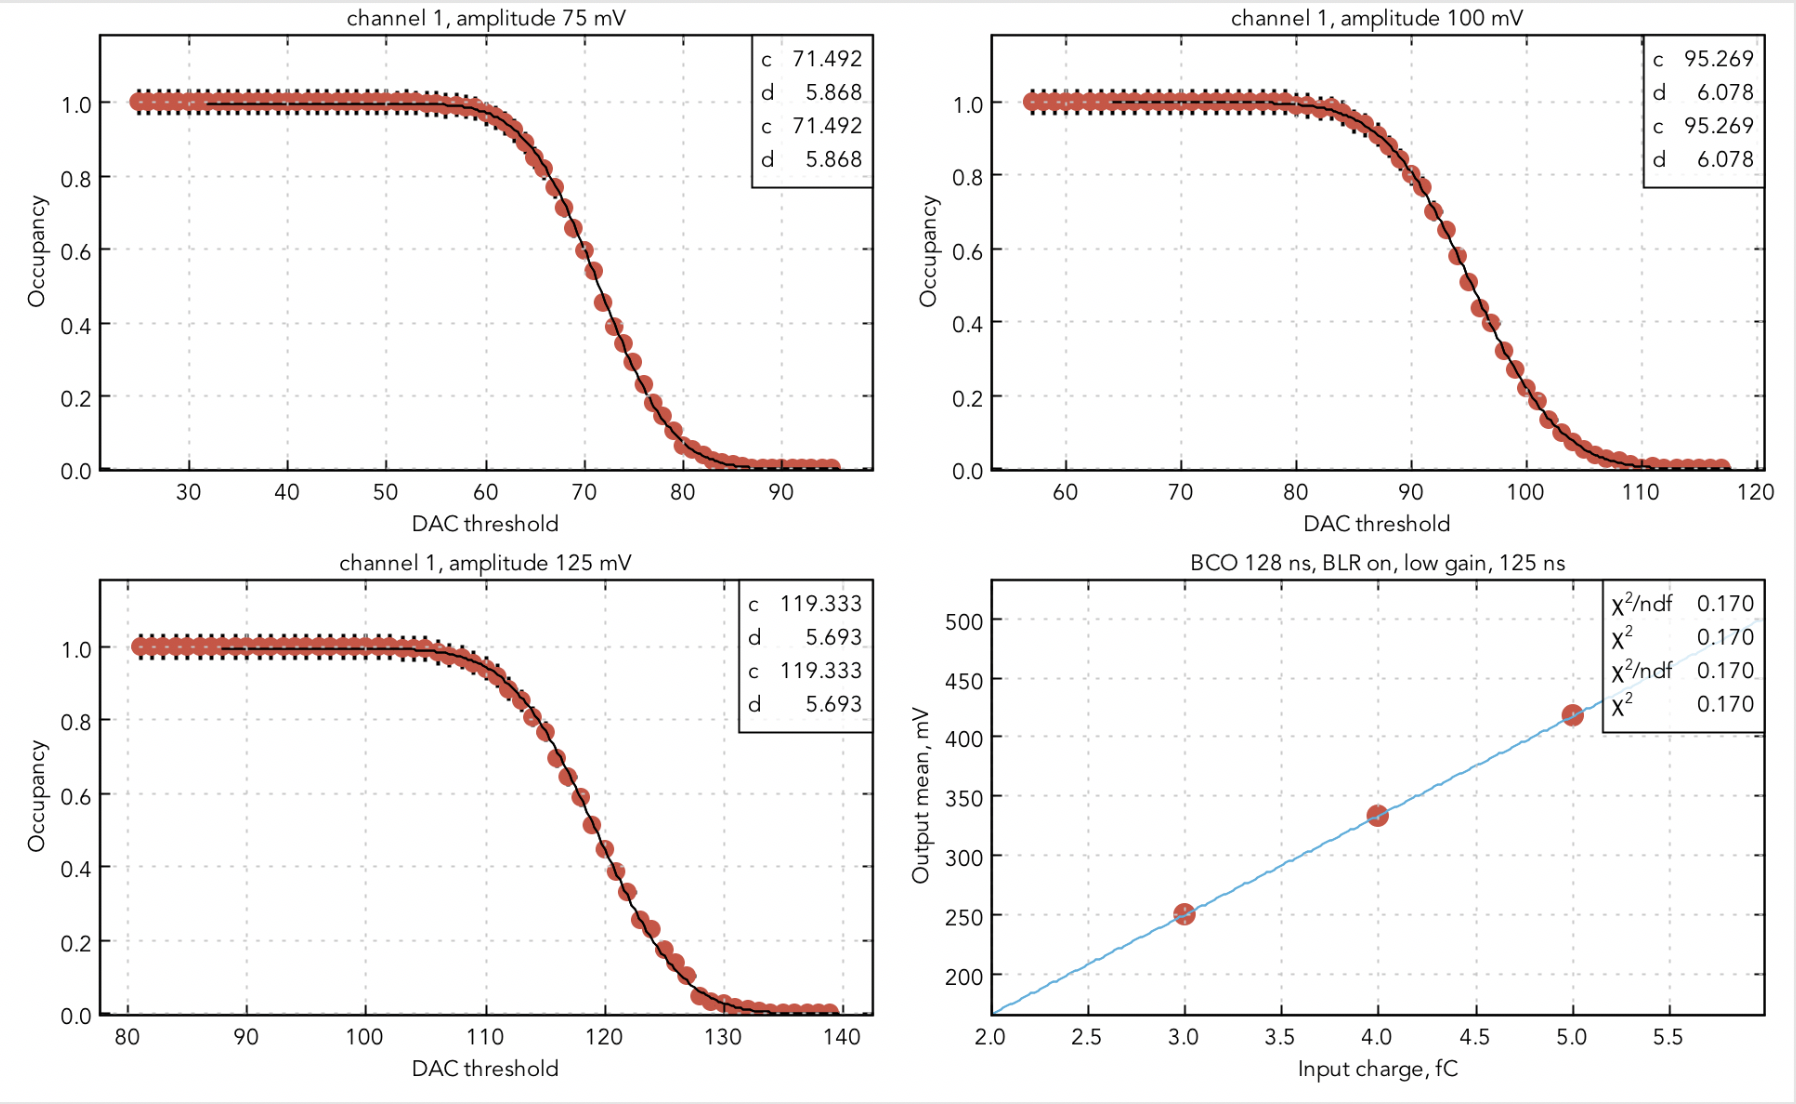
\includegraphics[width=1.0\columnwidth,keepaspectratio]{threshold-scan.png}
	\caption{Threshold scan on a single representative SVT channel.}
	\label{fig:threshold-scan}
\end{figure}

The output signals from the FSSR2 chip can be converted to charge using either internal or external calibration pulses. Because external pulser can be set to higher frequency than internal pulser without affecting the calibration process, external pulser circuit was added to the HBCB and the VSCM. Noise is measured using external, low frequency calibration charge injected in the absence of signal. The injected charge is shaped and amplified in the analog circuitry to form an output signal. The discriminator threshold determines whether or not the output signal corresponded to a hit. The probability that the injected charge produces a hit depends on the setting of the discriminator threshold. The average hit probability is measured by repeating the process of injecting charges and counting the fraction of readout triggers that produced a hit. This measurement is repeated over a range of threshold settings to produce an occupancy plot. 

The occupancy plots are measured setting the pulser amplitude at fixed values and changing the comparator thresholds. Each point of an occupancy plot represents the percentage of times that the comparator fires for a certain value of injected charge. In Fig.~\ref{fig:threshold-scan} presented three occupancy plots taken at different pulser amplitudes and the response plot showing the linear dependence of the output pulse height on the input charge in the operation region of the preamplifier. In between the high and low threshold regions, the occupancy curve is described by an error function, or S-curve, which can be fitted to the occupancy histogram for each channel, producing a mean value (discriminator threshold) and standard deviation (noise). The conversion from mV to electrons is performed considering a nominal value for the FSSR2 injection capacitance of 40~fF. 

\begin{figure}[hbt] 
	\centering 
	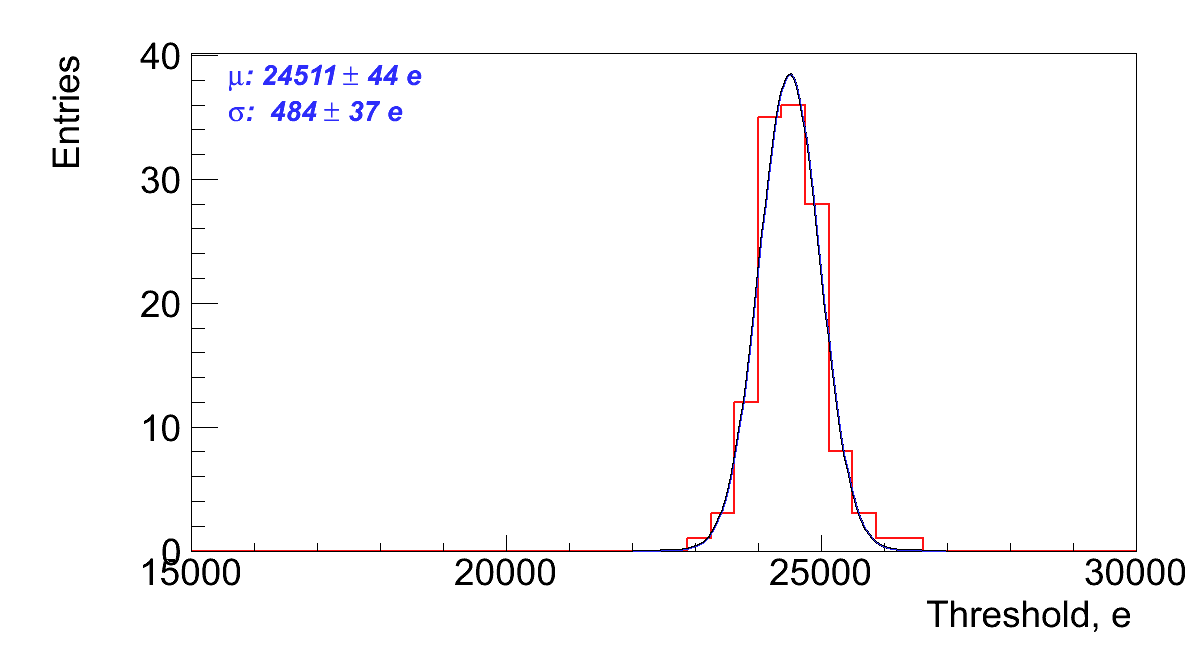
\includegraphics[width=0.8\columnwidth,keepaspectratio]{thrdisp.png}
	\caption{Typical threshold dispersion within a chip.}
	\label{fig:thrdisp}
\end{figure}

Threshold charge must be the same across the channels in a detector, otherwise the track-finding algorithms would be biased by the potential extra hits. Any spread in the response among the different channels of a chip results in a spread of the efficiency and noise occupancy which degrades effective performance. This leads to a requirement that the channel-to-channel variations in threshold and noise are kept to a minimum. Threshold dispersion is defined to be a standard deviation of the distribution of means obtained from the parameters of the complementary error function fit. The noise and threshold dispersion constants for each individual detector channel are measured and the values are used by the zero-suppression algorithms implemented in the core logic of the FSSR2 and by calibration procedures to identify defective channels. A comparison of the noise for 33~cm strips with the threshold spread demonstrates that the threshold spread is negligible compared to the noise and does not affect the efficiency and noise occupancy (see Fig.~\ref{fig:thrdisp}). The threshold dispersion agrees with expectations for the FSSR2 chip for the chosen settings.

SVT calibration data are stored in CLAS12 calibration database. The channel calibration table has columns corresponding to sector, layer, chip ID, mean, channel status (good, noisy, open, dead, or masked), ENC, gain, offset, V$_{t50}$ (threshold at 50$\%$ occupancy), and the threshold. There are 21504 rows in the channel calibration table. The ENC and gain are calculated using a calibration amplitude equal to 100 DAC.
The chip calibration table has columns corresponding to layer, sector, chip ID, ENC (electrons), gain (mV/fC), offset (mV), the threshold at 50$\%$ occupancy (V$_{t50}$, mV), threshold dispersion (electrons), chip gain (low, high), BLR mode (off, on), BCO time (ns), shaper time (ns), 8 ADC thresholds in DAC. There are 168 rows in the chip calibration table. 


\section{Detector Simulations}

Detailed simulations of the FT have been done with the Geant4-based Monte Carlo code for CLAS12,
GEMC~\cite{gemc} to optimize the detector design, to develop the reconstruction algorithms, and to understand
the detector performance.

Details on the implementation in GEMC of the detector geometry and digitization are reported in Ref.~\cite{gemc},
while an extensive discussion of the simulation studies that guided the detector design are presented in
Ref.~\cite{ft-tdr}. Here we focus on summarizing the results of the simulation studies that are relevant to
understand the FT performance.

\subsection{Leakage Corrections}

The reconstructed cluster energy can be systematically smaller than the actual energy of the particle that
induced the shower due to leakages in the shower containment caused by the limited dimensions of the
calorimeter, by cuts in the clustering algorithms, and thresholds in the hit detection. An example of the difference
between the reconstructed cluster energy and the simulated electron energy is shown in the top panel of
Fig.~\ref{fig:gemc_leakage}. This was obtained assuming an equivalent threshold on  the individual crystals of
10~MeV: the leakage varies from $\sim$80~MeV (16\%) for 500~MeV electrons to $\sim$300~MeV (6.6\%) for
4.5~GeV electrons.

This effect can be easily corrected for by parameterizing the leakage as a function of the reconstructed cluster
energy and position, and applying the correction in reconstruction. Simulations of single electrons were performed
in GEMC and the difference between the reconstructed cluster energy and the electron energy was studied as a
function of the cluster seed crystal. For each crystal, the dependence of this difference on the reconstructed
cluster energy was fitted to a fourth-order polynomial function, which was then used as an additive correction to
the reconstructed cluster energy. The final dependence of the difference between corrected cluster energy and
simulated energy is shown in the bottom panel of Fig.~\ref{fig:gemc_leakage}.

\begin{figure}
\includegraphics[height=\columnwidth]{fig/gemc_leakage.eps}
\caption{Top: difference between the simulated electron energy and the reconstructed cluster energy as a function
  of the electron energy for a 10~MeV equivalent threshold on the single crystal signal. Bottom: difference between
  the simulated electron energy and the cluster energy after the leakage correction.}
\label{fig:gemc_leakage}
\end{figure}

\subsubsection{Electromagnetic Background and Radiation Dose}

The electromagnetic background produced by the interaction of the electron beam in the target  at the nominal
CLAS12 luminosity was simulated in GEMC. For this purpose, in each event, about 124k, 11~GeV electrons were
generated that originated 10~cm upstream the target. The electrons were distributed randomly with the
radio-frequency structure of the beam in a 250~ns window. This number of electrons corresponds to the number
of beam electrons that would pass through the target in the chosen time window at the nominal CLAS12 luminosity
of 10$^{35}$~cm$^{-2}$s$^{-1}$. These simulations were used to study background rates in each of the FT detectors,
to determine the pile-up probability, and to estimate the radiation dose the FT would be subject to during operations.

The overall particle rate in the FT was found to be about 120~MHz, dominated by very low energy particles and with
only 6\% due to particles with energy above 100~MeV. In the energy range to be tagged (0.5-4.5~GeV) the overall
particle rate is further reduced to about 180~kHz, equally shared between photons and hadrons. 

For the FT-Cal, the energy deposition in each crystal was evaluated from the background simulation and used to
calculate the dose per unit of time. The overall radiation dose at $10^{35}$~cm$^{-2}$s$^{-1}$ was estimated to be
less than 1.5~rad/hr when averaged over the entire calorimeter with a distribution on the calorimeter crystals as
shown by Fig.~\ref{fig:ft_rad}. The maximum dose per crystal is of about 3~rad/hr, which would result in an
maximum integrated dose per crystal of about 2160~rad in 30~days of beam time.

\begin{figure}
\includegraphics[height=\columnwidth]{fig/ft_rad.eps}
\caption{Radiation dose on the FT calorimeter crystals in rad/hour at $10^{35}$~cm$^{-2}$s$^{-1}$ luminosity. The
  maximum values of about 5~rad/hr are observed for the innermost crystals, i.e. at the smaller angles.}
\label{fig:ft_rad}
\end{figure}

\section{Event Reconstruction}

Reconstruction of the FT sub-detector information and the matching between the detectors to determine the type and
three-momentum of the incident particles is implemented in the CLAS12 Java reconstruction framework. Details on
the algorithms and implementation are provided in Ref.~\cite{reconstruction}. In the following we briefly summarize
the main steps and final outputs.

FT-Cal hits are reconstructed from the analysis of the recorded FADC information to extract energy and time;
hits are then associated based on position and time to form clusters whose energy and centroid position are used
as an initial seed to define the three-momentum of the incident particles. Similarly, FT-Hodo hits are reconstructed
from the FADC raw information and matched based on position and timing to form clusters of matching tiles in the
two layers of the detector. These are matched to clusters in the calorimeter based on position and time to distinguish
charged particles from neutrals. Finally, FT-Trk hits are also reconstructed from the raw data and geometrically
grouped to form clusters in each of the detector layers separately. Combinations of clusters in the $x-y$ layers of
each of the two sub-detectors are used to define crosses that are finally matched to calorimeter clusters to improve
the determination of the impact point of the particle.


\section{Performance}The HTCC is one of the major CLAS12 systems used in experiments with the electron beam. The most important aspects of the HTCC performance are that it provides good timing, high electron detection efficiency, high signal strength, and high rejection factor of charged pions. All these parameters are critical for the quality of the data obtained in experiments since the detector, in combination with the forward calorimeter [ref. to ECAL], provides a fast trigger signal for CLAS12. As shown in section 6 the MC prediction for the HTCC for electrons is $\approx$100\%. Fig.~\ref{fig:RAFO_2GeV}. shows the experimentally measured electron detection efficiency for elastically scattered electrons at 2 GeV. The corresponding thresholds applied were approximately 2.5 photoelectrons. Measurements were performed using a special procedure with a random trigger that was not correlated with the HTCC. There were observed 27 events not detected by the HTCC due to the applied threshold. As shown, the electron detection efficiency is $\eta$ = (99$\pm$0.2)\%, which is in good agreement with the MC estimate. This result can be considered as a conservative estimate due to relatively high threshold used in measurements. Moreover, electrons travel a longer distance in the radiator gas (10 \% to 30 \% difference depending on a scattering angle). For these electrons the signal strength is higher, and therefore the detection efficiency is higher also as compared with the aforementioned efficiency for the elastically scattered electrons.   

\begin{figure}[!ht]
    \centering
    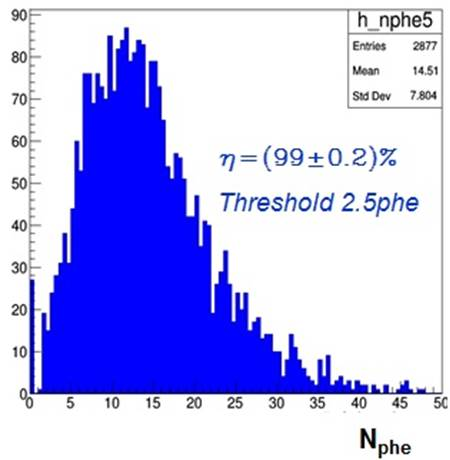
\includegraphics[width=1.0\linewidth,trim={0.0cm 0.0cm 0.0cm 0.0cm},clip]{images/RAFO_2GeV.jpg}
    \caption{Electron detection efficiency for elastically scattered electrons at 2 GeV. Data are obtained with the random trigger not correlated with the HTCC or other detector components of CLAS12.}
    \label{fig:RAFO_2GeV}
\end{figure}

Fig.~\ref{fig:positivePNPEC6595} shows the response of the detector in a wide range of particle momentum. The increase of number of events at high momenta is due to registration of charged pions (above threshold of their registration in the HTCC) and this is clearly illustrated.

\begin{figure}[!ht]
    \centering
    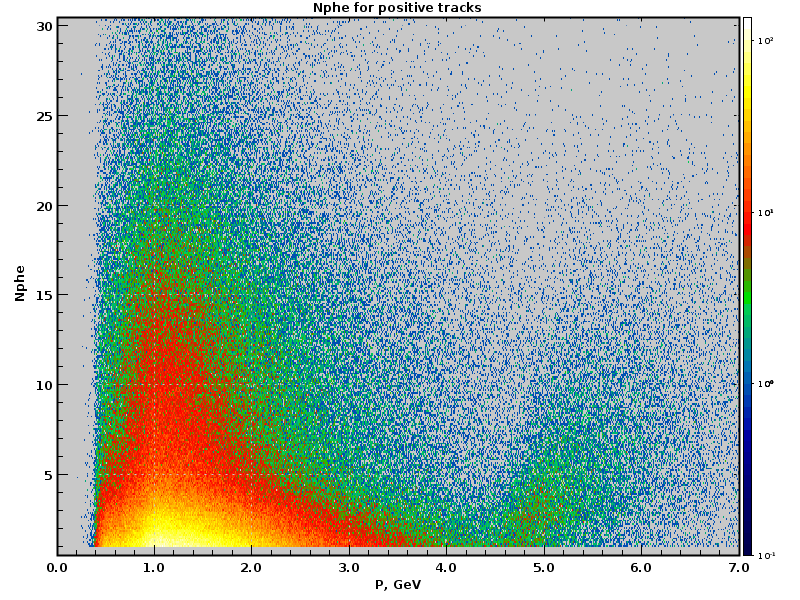
\includegraphics[width=1.0\linewidth,trim={0.0cm 0.0cm 0.0cm 0.0cm},clip]{images/positivePNPEC6595.png}
    \caption{Distributions of the HTCC response in a wide momentum range, including the region beyond the threshold of charged pion registration. Data obtained for positrons and $\pi^{+}$-mesons.}
    \label{fig:positivePNPEC6595}
\end{figure}

\begin{comment}
As shown bellow in the Fig.~\ref{fig:avgNPE_Theta_Phi_Dev_Build-2_NO_HOLES} the signal strength goes up for the utmost mirrors (large electron scattering angles). This is because electrons travel a longer distance in the radiator gas (10\% to 30\% difference depending on angle.) In other words the electron detection efficiency obtained for elastically scattered electrons at 2 GeV can be considered as as a conservative estimate for the efficiency of electron detection at larger angles.
\end{comment} 

The signal strength in the HTCC depends on the actual properties of the mirror facets, such as their final shape and reflectance. The accuracy of the combined mirror assembly and the alignment of the HTCC components (mirror, PMTs, Winston Cones), and the composition of the radiator gas all influence the final results. The FADC histogram of  the typical signal strength distribution obtained in one half-sector \#1 and \#2 of Sector 1 is shown in Fig.~\ref{fig:Signal_S1_HS1_HS2_R1_R2}. The signal strength for scattered electrons averaged over all HTCC channels is shown in Fig.~\ref{fig:Average_HTCC_Signal}. The experimentally measured mean value of 16.3 phe is close to Monte-Carlo simulation results, (see Fig.~\ref{fig:10cm_Targ_5T_Field_Phi}).

\begin{figure}[!ht]
    \centering
    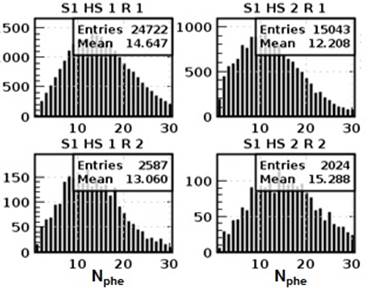
\includegraphics[width=1.0\linewidth,trim={0.0cm 0.0cm 0.0cm 0.0cm},clip]{images/Signal_S1_HS1_HS2_R1_R2.jpg}
    \caption{Typical distributions of the signal strength in channels covering polar angles in the range of $5^\circ$ to $12.5^\circ$ (Ring 1) and $12.5^\circ$ to $20.0^\circ$ (Ring 2) within azimuthal interval of $60^\circ$.}
    \label{fig:Signal_S1_HS1_HS2_R1_R2}
\end{figure}

\begin{figure}[!ht]
    \centering
    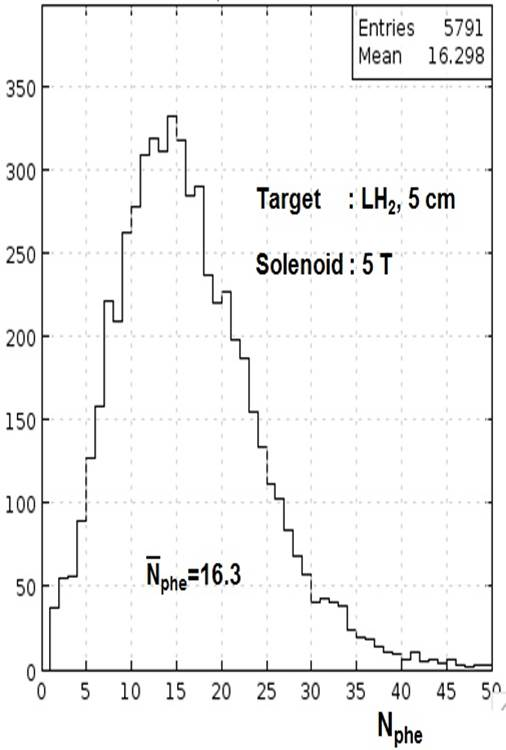
\includegraphics[width=1.0\linewidth,trim={0.0cm 0.0cm 0.0cm 0.0cm},clip]{images/Average_HTCC_Signal.jpg}
    \caption{The HTCC average signal strength for electrons from beam data.}
    \label{fig:Average_HTCC_Signal}
\end{figure}

Fig.~\ref{fig:HTCC_Response_run4013} shows the HTCC response for different electron momenta. Fig.~\ref{fig:avgNPE_Theta_Phi_Dev_Build-2_NO_HOLES}  shows the distribution of the HTCC response over the entire face of the mirror in the $x-y$-plane. Similar distribution is shown in Fig.~\ref{fig:avgNPE_XY_Dev_Build_02npe} obtained at the lower electron detection threshold of 0.2 photoelectrons. At the large electron scattering angles in range of 27.5$^\circ$ to 35$^\circ$, the statistics is lower. Fig.~\ref{fig:statistics_Theta_Phi_Dev_Build_NO_HOLES} shows the distribution of statistics in all 6 sectors. The data shows that the integrated signal strength is about 16.5 photoelectrons.

\begin{figure}[!ht]
    \centering
    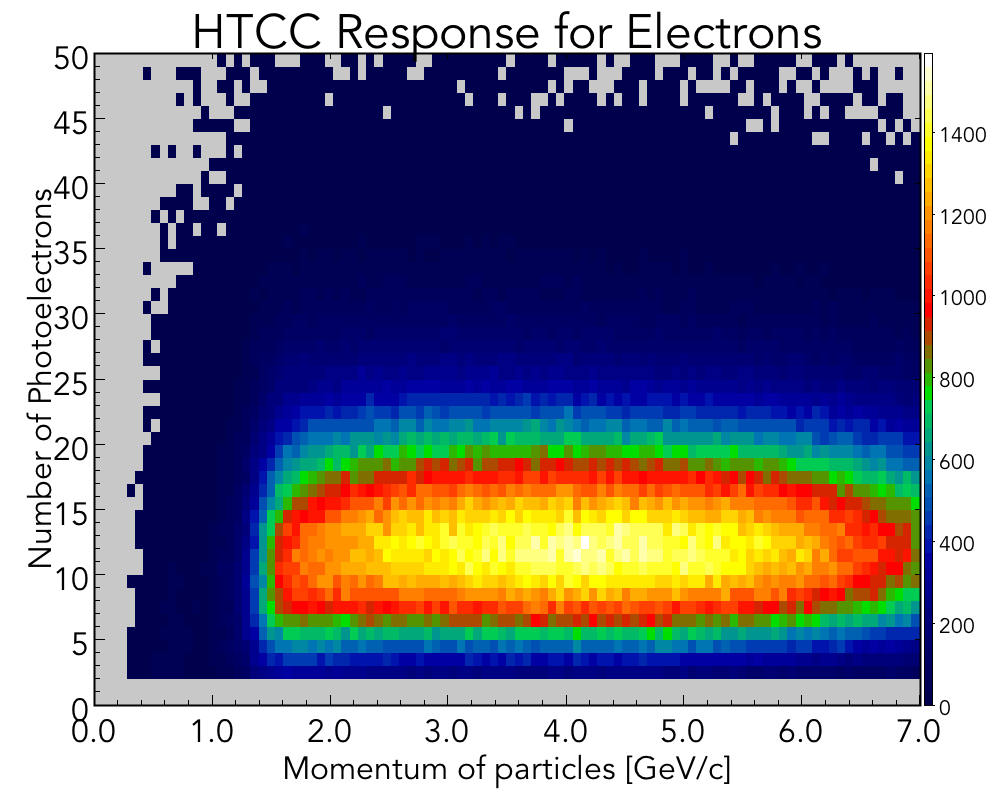
\includegraphics[width=1.0\linewidth,trim={0.0cm 0.0cm 0.0cm 1.73cm},clip]{images/HTCC_Response_run4013.png}
    \caption{The HTCC response for electrons: signal strength vs. momentum at 10.6 GeV energy.}
    \label{fig:HTCC_Response_run4013}
\end{figure}

\begin{figure}[!ht]
    \centering
    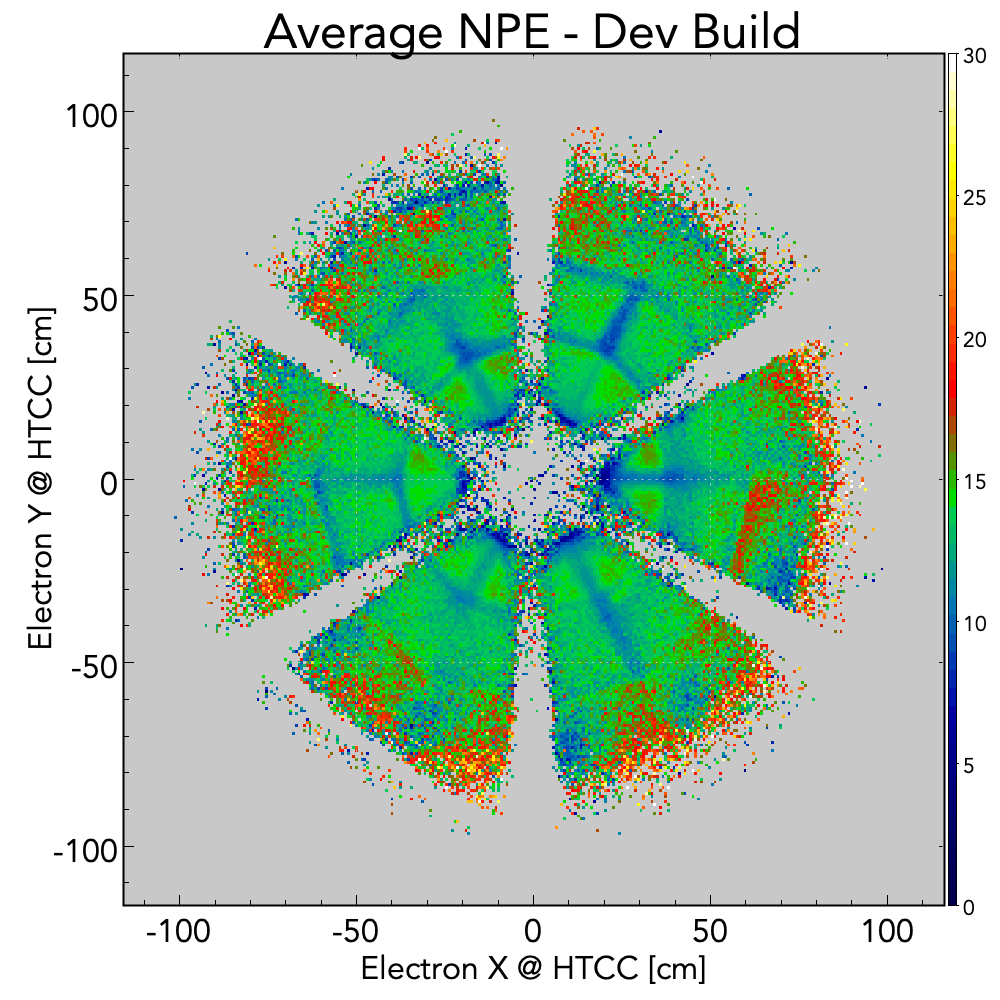
\includegraphics[width=1.0\linewidth,trim={0.0cm 0.0cm 0.0cm 1.67cm},clip]{images/avgNPE_Theta_Phi_Dev_Build-2_NO_HOLES.png}
    \caption{The HTCC response (in $N_{phe}$) for electrons in $x-y$-plane of the mirror.}
    \label{fig:avgNPE_Theta_Phi_Dev_Build-2_NO_HOLES}
\end{figure}

\begin{figure}[!ht]
    \centering
    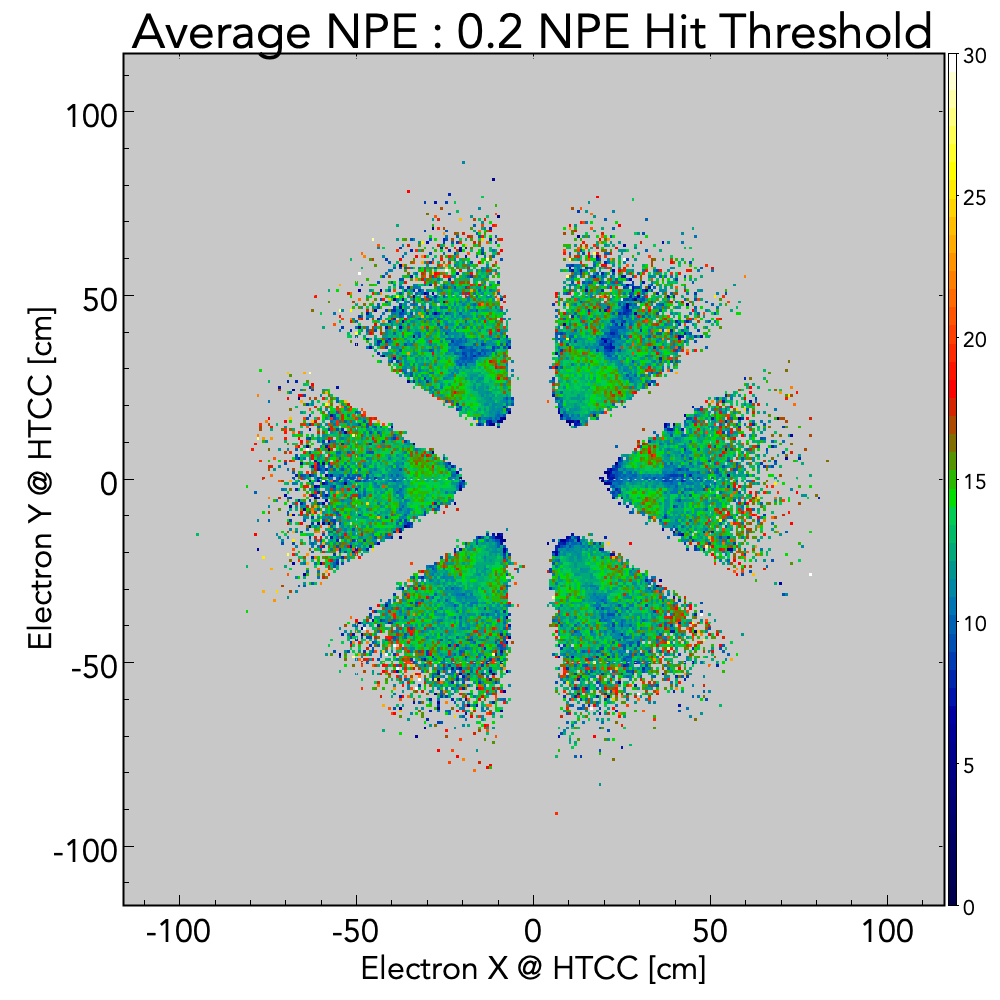
\includegraphics[width=1.0\linewidth,trim={0.0cm 0.0cm 0.0cm 1.67cm},clip]{images/avgNPE_XY_Dev_Build_02npe.png}
    \caption{The HTCC response (in $N_{phe}$) for electrons in $x-y$-plane of the mirror at the electron detection threshold of 0.2 photoelectrons.}
    \label{fig:avgNPE_XY_Dev_Build_02npe}
\end{figure}

\begin{figure}[!ht]
    \centering
    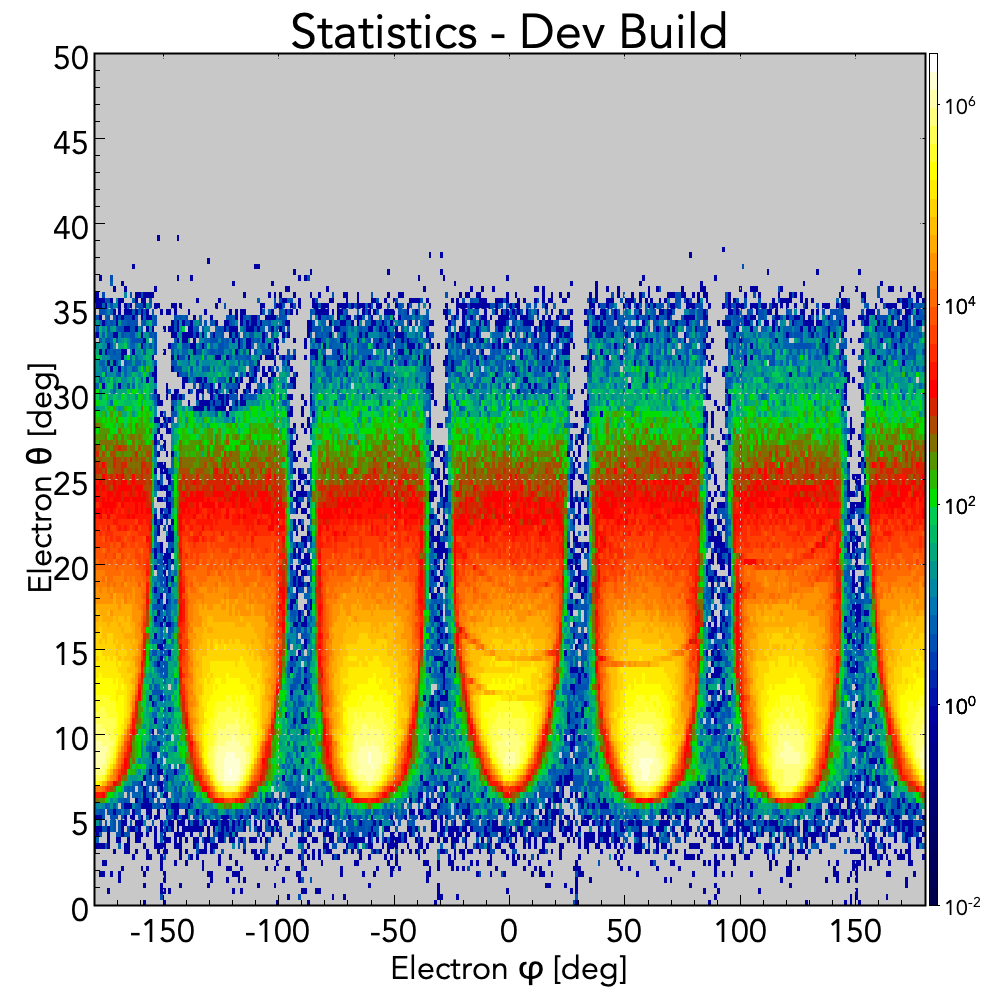
\includegraphics[width=1.0\linewidth,trim={0.0cm 0.0cm 0.0cm 1.67cm},clip]{images/statistics_Theta_Phi_Dev_Build_NO_HOLES.png}
    \caption{Distribution of statistics in all 6 sectors.}
    \label{fig:statistics_Theta_Phi_Dev_Build_NO_HOLES}
\end{figure}

We also note that in cases when the electrons cross the mirror close to its edges (at approximately at 5$^\circ$ and 35$^\circ$) one should expect unavoidable losses in the signal strength: some part of the Cherenkov light just passes by the mirror. As far as the internal borders between adjacent mirrors are concerned, there are similar losses that take place and are finally partially compensated due to the complete azimuthal symmetry of the detector, see Fig.~\ref{fig:avgNPE_Theta_Phi_Dev_Build-2_NO_HOLES}. The width of that area along internal boundaries that is deformed in the direction normal to the mirror face due to the shrinkage of the glue is estimated between $\sim$5 to $\sim$10 mm. This area includes the technological zone ~0.5 mm of width that is not reflecting the light at all. As a result these regions (width up to $\sim$10 mm) along internal boundaries between mirror facets defuse the light impinging the area, and therefore the signal strength is reduced. this edge effect is normal for the given design of the detector.


\section{Conclusions}

We have presented the software framework and event reconstruction that are currently being utilized for the processing of data collected by the CLAS12 experiment, in Hall B at Jefferson Lab.  

The framework was developed to allow processing of CLAS12 data for reconstruction and analysis purposes with an elastic, eclectic, and expandable approach thanks to the service-oriented architecture. The specific software applications leverage on an extensive set of common libraries for handling I/O, geometry, databases and magnetic field, designed to support data monitoring, calibration, reconstruction and analysis.

Full event reconstruction is implemented in the framework as a chain of micro-services that perform reconstruction of the individual CLAS12 sub-systems and whose output information is collected by the Event Builder service to form and identify particles. While the current reconstruction chain already supports reconstruction of all the sub-system and creation of full events, upgrades to the existing software implementation and algorithms are being studied.
\section*{Acknowledgments}

The authors would like to thank the engineering and technical staff of Jefferson Lab, the Italian Istituto
Nazionale di Fisica Nucleare, the University of Edinburgh, and the University of Glasgow, for their efforts
and support during the design, construction, and operation of the Forward Tagger. Special thanks to Gianni Nobili,
Andrea Rottura, and Diego Torazza for their assistance in this project. Many achievements in the development of the Forward
Tagger system would have not beem possible without the support of Nathan Baltzell, Sergey Boyarinov, Chris Cuevas,
Gagik Gavalian, Ben Raydo, Maurizio Ungaro, and Veronique Ziegler. This work was supported in part by the Italian
Istituto Nazionale di Fisica Nucleare, the Scottish Universities Physics Alliance (SUPA), the United Kingdom's Science
and Technology Facilities Council, the French Commissariat \`{a} l'Energie Atomique, the U.S. Department of Energy,
Office of Science, Office of Nuclear Physics under contract DE-AC05-06OR23177, the National Science Foundation
(ADD MRI DETAILS). 



\section*{References}
\bibliography{mybibfile}
\end{document}